%% 
%% Copyright 2007-2025 Elsevier Ltd
%% 
%% This file is part of the 'Elsarticle Bundle'.
%% ---------------------------------------------
%% 
%% It may be distributed under the conditions of the LaTeX Project Public
%% License, either version 1.3 of this license or (at your option) any
%% later version.  The latest version of this license is in
%%    http://www.latex-project.org/lppl.txt
%% and version 1.3 or later is part of all distributions of LaTeX
%% version 1999/12/01 or later.
%% 
%% The list of all files belonging to the 'Elsarticle Bundle' is
%% given in the file `manifest.txt'.
%% 
%% Template article for Elsevier's document class `elsarticle'
%% with harvard style bibliographic references

% \documentclass[preprint,12pt,authoryear]{elsarticle}

%% Use the option review to obtain double line spacing
%% \documentclass[authoryear,preprint,review,12pt]{elsarticle}

%% Use the options 1p,twocolumn; 3p; 3p,twocolumn; 5p; or 5p,twocolumn
%% for a journal layout:
%% \documentclass[final,1p,times,authoryear]{elsarticle}
% \documentclass[final,1p,times,twocolumn,authoryear]{elsarticle}
% \documentclass[final,3p,times,authoryear]{elsarticle}
% \documentclass[final,3p,times,twocolumn,authoryear]{elsarticle}
% \documentclass[final,5p,times,authoryear]{elsarticle}
\documentclass[final,5p,times,twocolumn,authoryear]{elsarticle}

%% For including figures, graphicx.sty has been loaded in
%% elsarticle.cls. If you prefer to use the old commands
%% please give \usepackage{epsfig}

% \usepackage{balance}
\def\pub{false} % true for publication, false for draft
\newcommand*{\template}{template}
\input{\template/preamble/preamble_Elsevier.tex}

\newcommand*{\figSizeTwoCol}{.49}
\newcommand*{\figSizeOneCol}{0.98}

% %% The amssymb package provides various useful mathematical symbols
% \usepackage{amssymb}
% %% The amsmath package provides various useful equation environments.
% \usepackage{amsmath}
% %% The amsthm package provides extended theorem environments
% %% \usepackage{amsthm}

%% The lineno packages adds line numbers. Start line numbering with
%% \begin{linenumbers}, end it with \end{linenumbers}. Or switch it on
%% for the whole article with \linenumbers.
%% \usepackage{lineno}

\journal{Nuclear Physics B}

\begin{document}

\begin{frontmatter}

%% Title, authors and addresses

%% use the tnoteref command within \title for footnotes;
%% use the tnotetext command for theassociated footnote;
%% use the fnref command within \author or \affiliation for footnotes;
%% use the fntext command for theassociated footnote;
%% use the corref command within \author for corresponding author footnotes;
%% use the cortext command for theassociated footnote;
%% use the ead command for the email address,
%% and the form \ead[url] for the home page:
%% \title{Title\tnoteref{label1}}
%% \tnotetext[label1]{}
%% \author{Name\corref{cor1}\fnref{label2}}
%% \ead{email address}
%% \ead[url]{home page}
%% \fntext[label2]{}
%% \cortext[cor1]{}
%% \affiliation{organization={},
%%            addressline={}, 
%%            city={},
%%            postcode={}, 
%%            state={},
%%            country={}}
%% \fntext[label3]{}

\title{
  Constrained Optimization-Based Neuro-Adaptive Control (CoNAC) for Uncertain Euler-Lagrange Systems Under Weight and Input Constraints 
} %% Article title

%% use optional labels to link authors explicitly to addresses:
%% \author[label1,label2]{}
%% \affiliation[label1]{organization={},
%%             addressline={},
%%             city={},
%%             postcode={},
%%             state={},
%%             country={}}
%%
%% \affiliation[label2]{organization={},
%%             addressline={},
%%             city={},
%%             postcode={},
%%             state={},
%%             country={}}

\author{
  Myeongseok Ryu, Donghwa Hong, and Kyunghwan Choi
} %% Author name

%% Author affiliation
\affiliation{organization={
  Department of Mechanical and Robotics Engineering, Gwangju Institute of Science and Technology (GIST)
},%Department and Organization
            addressline={123 Cheomdangwagi-ro, Buk-gu}, 
            city={Gwangju},
            postcode={61005}, 
            % state={},
            country={Korea}}

%% Abstract
\begin{abstract}
  This study presents a constrained optimization-based neuro-adaptive controller (CoNAC) for uncertain Euler-Lagrange systems subject to weight norm and input constraints. A deep neural network (DNN) is employed to approximate the ideal stabilizing control law, compensating for lumped system uncertainties while addressing both types of constraints. The weight adaptation laws are formulated through a constrained optimization problem, ensuring first-order optimality conditions at steady state. The controller's stability is rigorously analyzed using Lyapunov theory, guaranteeing bounded tracking errors and DNN weights. Numerical simulations comparing CoNAC with three benchmark controllers demonstrate its effectiveness in tracking error regulation and satisfaction of constraints.
\end{abstract}

%%Graphical abstract
\begin{graphicalabstract}
%\includegraphics{grabs}
\end{graphicalabstract}

%%Research highlights
\begin{highlights}
\item Research highlight 1
\item Research highlight 2
\end{highlights}

%% Keywords
\begin{keyword}
Neuro-adaptive control \sep constrained optimization \sep deep neural network \sep Euler-Lagrange system \sep input constraint

%% keywords here, in the form: keyword \sep keyword
%% PACS codes here, in the form: \PACS code \sep code

%% MSC codes here, in the form: \MSC code \sep code
%% or \MSC[2008] code \sep code (2000 is the default)

\end{keyword}

\end{frontmatter}

%% Add \usepackage{lineno} before \begin{document} and uncomment 
%% following line to enable line numbers
%% \linenumbers

%% main text
%%


\section*{Notation}
In this study, the following notation is used:

\begin{itemize}
    \item $\otimes$ denotes the Kronecker product \cite[Definition 7.1.2]{Bernstein:2009aa}.
    \item $\mv x=[x_i]_{i\in[1,\cdots,n]}\in\R^n$ and $
        \mm A
        := 
        [a_{ij}]
        _{
            i\in[1,\cdots,n],j\in[1,\cdots ,m]
        }\allowbreak\in\R^{n\times m}
        $ denote a vector and a matrix.
    \item $\myrow_i(\mm A)$ denotes the $i\textsuperscript{th}$ row of the matrix $\mm A\in\R^{n\times m}$. 
    \item $\myvec(\mm A):= [\myrow_1(\mm A^\top)  ,\cdots,\myrow_m(\mm A^\top)  ]^\top   $ for $\mm A\in\R^{n\times m}$.
    % \item $\mycol_i(A)$ and $\myrow_j(A)$ denote the $i\textsuperscript{th}$ column and $j\textsuperscript{th}$ row of $A\in\R^{n\times m}$, respectively.
    % \item $\myvec(A):= [\mycol_1(A)^\top  ,\cdots,\mycol_m(A)^\top  ]^\top   $ for $A\in\R^{n\times m}$.
    \item $\lambda_{\min}(\mm A)$ denotes the minimum eigenvalue of the matrix $\mm A\in\R^{n\times n}$.
    \item $\mm I_n$ denotes the $n\times n$ identity matrix, and $\mm 0_{n\times m}$ denotes the $n\times m$ zero matrix.
\end{itemize}

%  SECTION INTRODUCTION ===================================
\section{Introduction}

\subsection{Background}

Many engineering systems, including those in aerospace, robotics, and automotive applications, can be modeled using Euler-Lagrange systems. 
These systems are governed by dynamic equations derived from energy principles and describe the motion of mechanical systems with constraints. 
In practice, however, such systems often exhibit uncertainties due to unmodeled dynamics, parameter variations, or external disturbances. 
These uncertainties can significantly degrade control performance and, in some cases, lead to instability. 
To address these challenges, adaptive control methods have been widely employed to ensure robust performance in the presence of system uncertainties \cite{Ioannou:2006aa, Tao:2003aa}.

More recently, neuro-adaptive control approaches have been introduced to approximate unknown system dynamics or entire control laws using neural networks (NNs) \cite{Farrell:2006aa}. 
NNs are well-known for their universal approximation property, which allows them to approximate any smooth function over a compact set with minimal error. 
Various types of NNs have been utilized in neuro-adaptive control, including simpler architectures like single-hidden layer (SHL) neural networks \cite{Ge:2010aa, Yesildirek:1995aa} and radial basis function (RBF) neural networks \cite{Liu:2013ab,Ge:2002aa}, as well as more complex models like deep neural networks (DNNs) \cite{Patil:2022aa} and their variations. 
SHL and RBF NNs are often employed to approximate uncertain system dynamics or controllers due to their simplicity \cite{Esfandiari:2014aa,Esfandiari:2015aa,Yesildirek:1995aa,Gao:2006aa}, while DNNs offer greater expressive power, making them more effective for complex system approximations \cite{Rolnick:2018aa}. 
Additionally, variations of DNNs, such as long short-term memory (LSTM) networks for time-varying dynamics \cite{Liu:2013ab} and physics-informed neural networks (PINNs) for leveraging physical system knowledge \cite{Hart:2024aa}, have further extended the capabilities of neuro-adaptive control systems.

A critical aspect of neuro-adaptive control is the weight adaptation law, which governs how NN parameters are updated. 
Most studies derived these laws using Lyapunov-based methods, ensuring the boundedness of the tracking error and weight estimation error, thus maintaining system stability under uncertainty.

However, two significant challenges persist in using NNs for adaptive control. 
First, the boundedness of NN weights is not inherently guaranteed, which can result in unbounded outputs. 
When NN outputs are used directly in the control law, this may lead to excessive control inputs, violating input constraints. 
Such constraints are commonly encountered in industrial systems, where actuators are limited by physical and safety requirements in terms of amplitude, rate, or energy \cite{Esfandiari:2021aa}. 
Failing to address these constraints can degrade control performance or even destabilize the system.

Therefore, addressing these two key issues—ensuring weight boundedness and satisfying input constraints—is essential for the reliable design of neuro-adaptive controllers. 
he following section will provide a detailed review of the existing solutions to these challenges.

\subsection{Literature Review}

\subsubsection{Ensuring Weight Norm Boundedness}

A common challenge in neuro-adaptive control is maintaining the boundedness of the NN weights to ensure stability. 
In many studies, projection operators were employed to enforce upper bounds on the weight norms, ensuring that the weights do not grow unboundedly. 
For example, in \cite{Zhou:2023aa,Griffis:2023aa,Patil:2022aa}, projection operators were used to constrain the weight norms to remain below predetermined constants. 
However, these constants were often selected as large as possible due to the lack of theoretical guarantees regarding the global optimality of the weight values. 
While this approach ensured that the NN remained stable, it did not necessarily result in optimal performance.

In addition to projection operators, some studies utilized modification techniques like $\sigma$-modification \cite{Ge:2002aa} and $\epsilon$-modification \cite{Esfandiari:2015aa,Gao:2006aa}. 
These methods ensured that the NN weights remained within an invariant set by incorporating stabilizing functions into the adaptation law. 
Although these techniques were effective in ensuring boundedness and avoiding weight divergence, they similarly lacked a formal analysis of the optimality of the adapted weights, leaving room for improvement in terms of performance optimization.

\subsubsection{Satisfying Input Constraints}

The second major issue is satisfying input constraints, particularly in systems where actuators are subject to physical limitations. 
The unpredictable outputs of NNs can sometimes lead to excessively large control inputs, violating these constraints. 
This problem is exacerbated in neuro-adaptive controllers that attempt to cancel out system dynamics using conventional methods like feedback linearization or backstepping. 
In such cases, controllers may produce overly aggressive control inputs, even when the system's natural dynamics are stabilizing, leading to unnecessary saturation of the control inputs.

To address input saturation, many studies introduced auxiliary systems. 
These systems mitigated the effects of control input saturation by modifying the control strategy when saturation occurred. 
For instance, in \cite{Esfandiari:2014aa,Karason:1994aa,Esfandiari:2015aa}, auxiliary states were generated whenever input saturation was detected, and these states were incorporated into the adaptation law to adjust the NN weights accordingly. 
This approach helped the controller reduce input saturation by indirectly regulating the auxiliary states.

Alternatively, auxiliary states can also be used as feedback terms in the control law to directly compensate for the effects of input saturation constraints, as demonstrated in \cite{Arefinia:2020aa,He:2016aa,Peng:2020aa}. 
In \cite{Gao:2006aa}, the NN was used to approximate the desired control input, compensating for input saturation. 
However, these approaches typically handle input bound constraints on a per-input basis (\ie applying bounds to each scalar control variable individually), and may not account for more complex, nonlinear constraints, like input norm constraints, which are commonly found in physical systems such as robotic actuators or motor systems.

\subsubsection{Limitations of Existing Approaches and Potential of Constrained Optimization}

Although both the projection operator methods for weight norm boundedness and the auxiliary system approach for input constraints have shown effectiveness, they come with significant limitations. 
Projection operators and modification techniques do not guarantee the optimality of the adapted weights. 
Moreover, auxiliary systems typically handle only simple forms of input constraints, such as input bound constraints, limiting their ability to address more complex, nonlinear constraints like input norm constraints.

To overcome these limitations, constrained optimization offers a promising approach. 
By formulating the neuro-adaptive control problem as an optimization problem with constraints, it is possible to adapt the NN weights while minimizing an objective function (\eg tracking error) subject to both weight norm and input constraints. 
Constrained optimization provides a theoretical framework for defining optimality and presents numerical methods for finding solutions that satisfy the constraints \cite{Nocedal:2006aa}.

In existing literature, constrained optimization techniques, such as the Augmented Lagrangian Method (ALM) \cite{Evens:2021aa} and the Alternating Direction Method of Multipliers (ADMM) \cite{Wang:2019aa,Taylor:2016aa}, have been used to train NNs offline. 
These methods impose constraints to address issues like gradient vanishing in backpropagation. 
However, to the best of the authors' knowledge, no prior work has applied constrained optimization to adaptive control systems with real-time weight adaptation. 
This gap suggests that constrained optimization could be key to addressing both weight norm boundedness and input constraints in a unified, theoretically grounded framework, particularly in real-time neuro-adaptive control.

\subsection{Contributions}

The main contributions of this study are listed as follows:
\begin{itemize}
    \item A constrained optimization-based neuro-adaptive controller (CoNAC) is developed using a DNN, where input constraints and the boundedness of NN weights are formulated as inequality constraints within the adaptation process.
    \item The weight adaptation laws in CoNAC are derived using constrained optimization theory to minimize the objective function while satisfying the inequality constraints. The adaptation laws ensure convergence of the weights to the first-order optimality conditions, specifically the Karush-Kuhn-Tucker (KKT) conditions.
    \item The forward sensitivity method is applied in CoNAC to accurately calculate the gradient of the objective function. \MSRY{WILL BE DELETED}
    %, enabling more precise real-time adaptation.
\end{itemize}

\subsection{Organization}

The remainder of this paper is organized as follows. 
Section \ref{sec:Problem Formulation} presents the target system and control objective.
Section \ref{sec:ctrl design} introduces the proposed controller and the architecture of DNN in the controller. 
In Section \ref{sec:adap_laws}, the weight adaptation laws are developed.
Candidates of input constraints are presented in \ref{sec:appen:cstr}.
Section \ref{sec:stability} analyzes the stability of the proposed controller.
A comparative study of the four selected controllers, including the proposed controller, is reported in Section \ref{sec:sim}.
Finally, Section \ref{sec:conclusion} concludes the paper and discusses potential future work.
% The appendices provide the proof of the lemma used in the stability analysis.

%  SECTION PROBLEM FORMULATION ============================
\section{Problem Formulation}\label{sec:Problem Formulation}

\subsection{Model Dynamics and Control Objective}

Consider an uncertain Euler-Lagrange system modeled as
\begin{equation}
    \rbM\ddq + \rbVm + \rbF + \rbG + \rbd
    =
    \mysat(\rbu)
    \label{eq:sys1}
\end{equation}
where $\q\in \R^n$ denotes the generalized coordinate, $\rbd$ represents disturbance and $\rbu\in\R^n$ denotes the control input. 
The terms $\rbM:=\rbM(\q)\in\R^{n\times n}$, $\rbVm:=\rbVm(\q,\dq)\in\R^{n\times n}$, $\rbF:=\rbF(\dq)\in\R^{n}$ and $\rbG:=\rbG(\q)$ represent the unknown inertia matrix, Coriolis/centripetal matrix, friction terms and gravity vector
The function $\mysat(\cdot):\R^n\to\R^n$ represents the inherent physical limitations of the actuators such that $\norm{\mysat(\rbu)}\le \overline\tau$, where $\overline\tau$ denotes the maximum norm of control input.
To account for these limitations, it is essential to incorporate physically motivated constraints into the controller design.
Appendix \ref{sec:appen:cstr} introduces candidate constraints that can be applied to ensure compliance with these physical limitations.

The Euler-Lagrange system \eqref{eq:sys1} satisfy some important physical properties \cite[see, Chap. 3 Tab. 3.2.1]{Lewis:1998aa}.
We introduce the following properties:
\begin{prop} 
    The inertia matrix $\rbM$ is symmetric, positive definite and bounded.
    \label{prop:M}
\end{prop}

\begin{prop} 
    The Coriolis/centripetal matrix $\rbVm$ can always be selected so that the matrix $(\dot{\rbM}-2\rbVm)$ is skew-symmetric.
    \label{prop:skew}
\end{prop}

\begin{prop}
    The disturbance $\rbd$ is bounded so that $\norm{\rbd}\le \overline\tau_d$.
    \label{prop:dis_bound}
\end{prop}

In conclusion, the control objective is to develop a neuro-adaptive controller that enables $\q$ to track a continuously differentiable desired trajectory $\qd:=\qd(t): \R \to \R^n$, compensating for the external disturbance while addressing the imposed constraints.
Considering the control input saturation function, $\qd(t)$ is supposed to satisfy the following assumption:
\begin{assum}
    The desired trajectory $\qd(t)$ is bounded so that $\norm{\qd(t)}\le \overline{q}_d$ and available to design a feasible control input in the presence of the control input saturation.
    \label{assum:feasible}
\end{assum}

%  SECTION CONTROLLER DESIGN ==============================
\section{Control Law Development}\label{sec:ctrl design}

The architecture of the proposed CoNAC is illustrated in Fig.~\ref{fig:ctrl:diagram}, consisting of: a DNN that functions as a neuro-adaptive controller, and a weight optimizer for the DNN. 
Section \ref{sec:sub:NAC} presents the neuro-adaptive controller along with the reference generator, and Section \ref{sec:sub:NN definition} defines the DNN model. The weight optimizer will be detailed in Section \ref{sec:sub:weight optimizer}.

\begin{figure*}[!t]
    \centering
    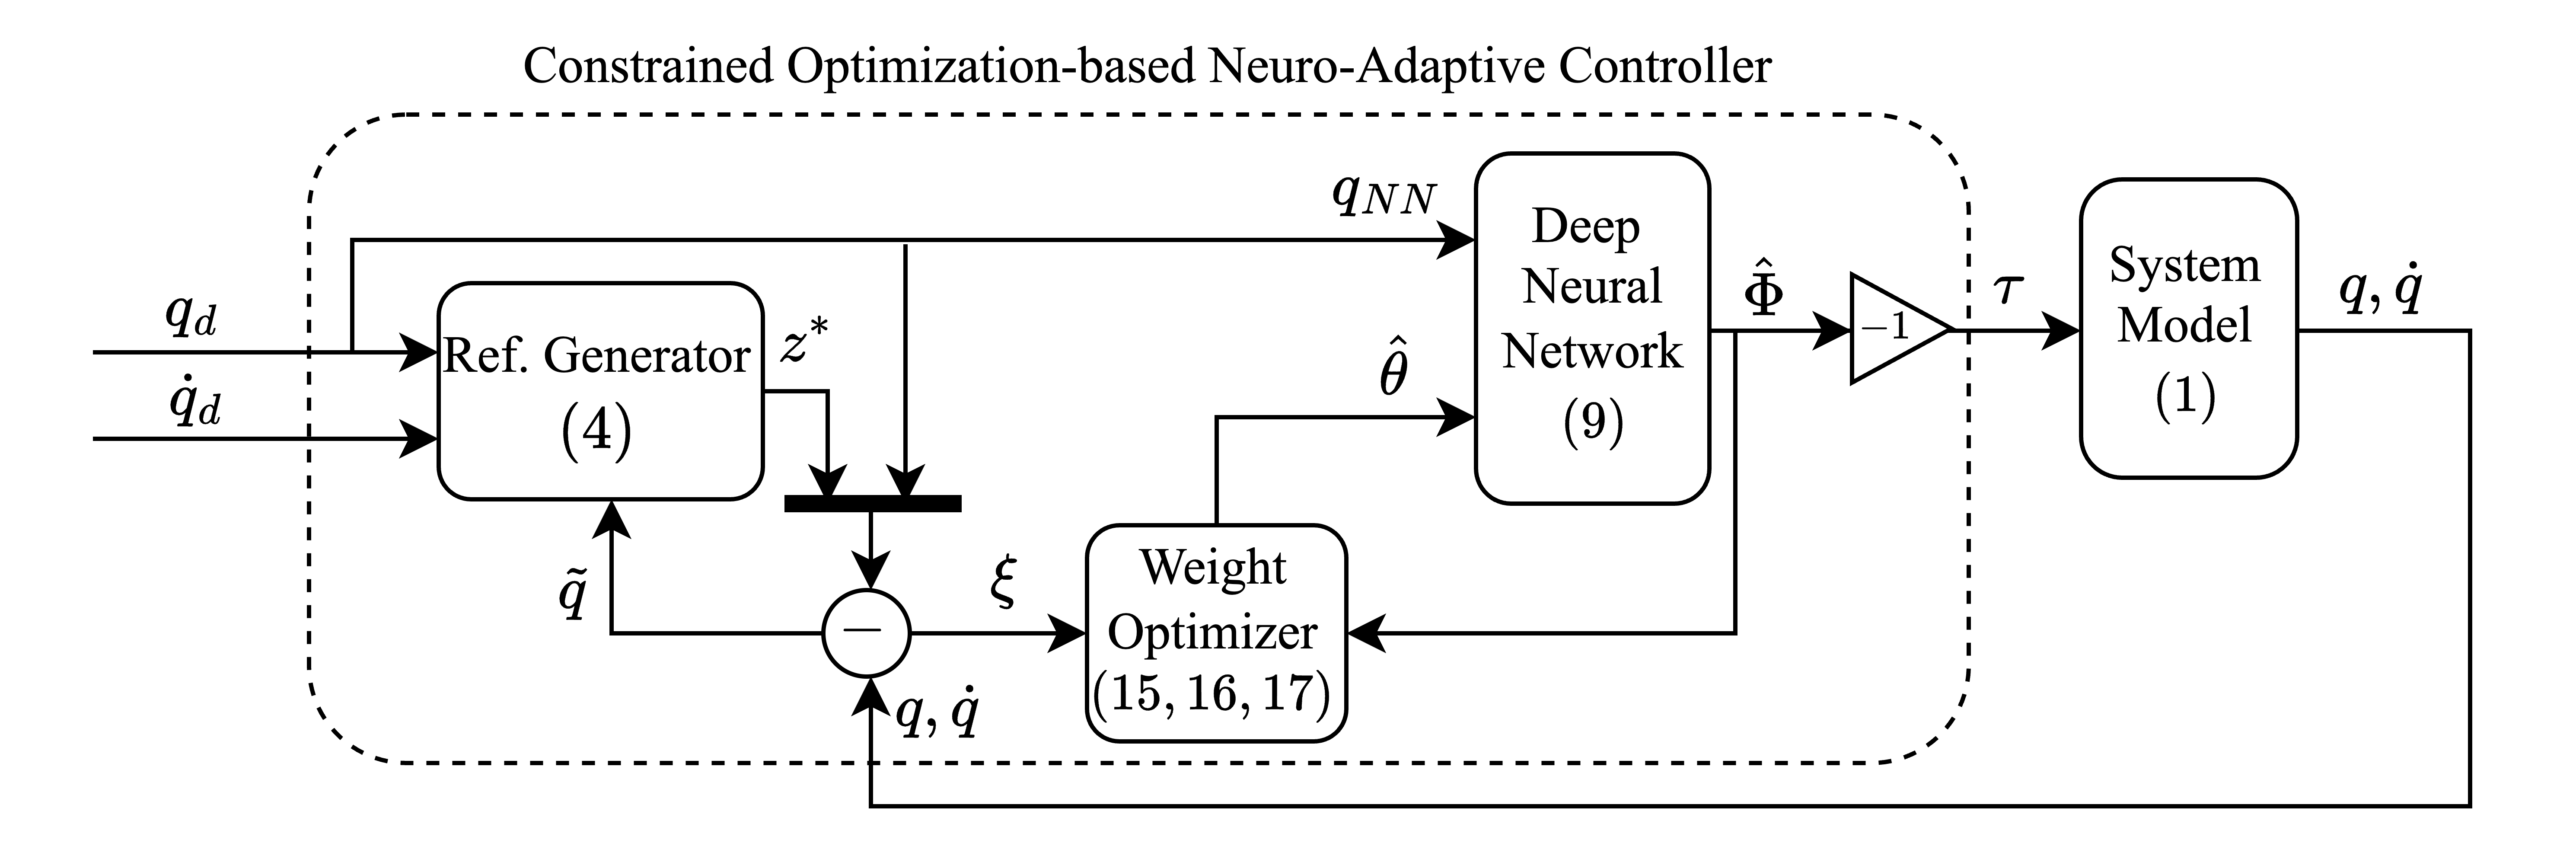
\includegraphics[width=0.8\linewidth]{src/figures/Controller.drawio.png}
    % \includesvg[width=0.75\linewidth]{Controller.drawio.svg}
    \caption{Architecture of the constrained optimization-based neuro-adaptive controller (CoNAC).}
    \label{fig:ctrl:diagram}
\end{figure*}

\subsection{Neuro-Adaptive Controller Design}\label{sec:sub:NAC}

First, let us define the filtered tracking error $\fe\in\R^n$ as 
\begin{equation}
    \fe := \dot{\mv e}-\mm\Lambda \mv e
    ,
    \label{eq:err:filtered}
\end{equation}
where $\mv e := \q - \qd$ denotes the tracking error, $\dot{\mv e} := \dq - \dqd$ represents the derivative of the tracking error, and $\mm\Lambda\in\R^{n\times n}_{>0}$ is a user-designed filtering matrix.
Since \eqref{eq:err:filtered} is stable system, it implies that $\mv e$ is bounded if $\fe$ is bounded.

Using $\fe$, the system dynamics \eqref{eq:sys1} can be rewritten as
\begin{equation}
    \rbM \dot\fe
    =
    -\rbVm \fe
    -\mm K \fe
    + \mv f
    -\rbd + \mysat(\rbu)
    ,
    \label{eq:sys:filtered}
\end{equation}
where $\mm K\in\R^{n\times n}$ denotes arbitrary symmetric positive definite matrix and $
    \mv f:= \mv f(\q,\dq,\dqd,\ddqd)
    =
    \mm K \fe
    +\rbM(-\ddqd+\mm\Lambda\dot{\mv e})
    +
    \rbVm(-\dqd+\mm\Lambda\mv e)
    -
    \rbF
    -
    \rbG
    \in\R^n
$ denotes the lumped system uncertainty.

Consider the Lyapunov function $V_1:= \tfrac{1}{2}\fe^\top \rbM\fe$. 
Invoking Property \ref{prop:skew}, the time derivative of $V_1$ is
\begin{equation}
    \begin{aligned}
        \ddtt{V}_1
        =&
        \fe^\top \rbM (
            -\rbVm \fe -\mm K \fe + \mv f
            -\rbd + \mysat(\rbu)
        )
        \\
        &
        +
        \tfrac{1}{2}
        \fe^\top \dot{\rbM}\fe
        \\
        =&
        -
        \fe^\top \mm K \fe 
        +
        \fe^\top (
            \mv f+\mysat(\rbu)
            -\rbd
        )
        \\
        &
        +
        \tfrac{1}{2}
        \fe^\top(\dot{\rbM}- 2\rbVm)\fe
        \\
        \le&
        -\lambda_{\min}(\mm K)\norm{\fe}^2
        +
        \overline\tau_d\norm{\fe}
        +
        \fe^\top (\mv f+\mysat(\rbu))
        \\
        \le&
        -\lambda_{\min}(\mm K)\norm{\fe}^2
        +
        \overline\tau_d\norm{\fe}
        +
        \fe^\top (\mysat(\rbu)-\rbu^*)
        ,
    \end{aligned}
    \label{eq:lya1:dot1}
\end{equation}
where $\rbu^*:= -\mv f$ is the ideal control input whose maximum norm is $\overline\tau$ according to Assumption \ref{assum:feasible} and $\mysat(\cdot)$. 
Therefore, one can conclude that $\fe$ is exponentially stable so that $\lim_{t\to\infty}\norm{\fe}=\tfrac{\overline\tau_d}{\lambda_{\min}(\mm K)}$, if $\rbu=-\rbu^*$ can be realized.
However, $\rbu^*$ is not available in practice, since $\mv f$ is unknown.
\MSRY{여기서는 MVT, IFT을 사용하지 않았기 때문에 아이디얼 제어가 포화되지 않을 필요성이 없다. 실험에서도 포화를 핸들링하는 중에 추종이 완벽히 되지 못하는 것을 보인다.}

To overcome this issue, a DNN is employed to approximate $\rbu^*$.
Let $\NN:=\NN({\q}_n;\wth): \R^{l}\times\R^{\Xi}\to\R^{n}$ represent the DNN, where ${\q}_n\in\R^{l}$ is the DNN input vector, and $\wth\in\R^{\Xi}$ is the vector of trainable weights.
The architecture of $\NN({\q}_n;\wth)$ will be defined in Section \ref{eq:DNN:architecture}.
According to the universal approximation theorem for DNNs \cite{Kidger:2020aa}, $\NN({\q}_n;\wth)$ can approximate a nonlinear function $\mv g(\cdot)$ with an ideal weight vector $\idealwth$ on a compact subset $\Omega_{NN}\in\R^{l}$ to $\mv\epsilon$-accuracy, such that $\sup_{{\q}_n\in\Omega_{NN}}\norm{ \NN({\q}_n;\idealwth) - \mv g(\cdot)} = \mv\epsilon < \infty$.
Furthermore, the theorem states that the norm of $\idealwth$ is bounded, \ie $\norm{\idealwth}\le \overline\wth<\infty$.
In this study, $\idealwth$ is defined as a local optimal point, rather than a global optimal point.

In conclusion, the ideal control law $\rbu^*$ is expressed by the DNN approximation with the ideal weight vector $\idealNN:=\NN({\q}_n;\idealwth)$ as follows:
\begin{align}
    \rbu^*=& \idealNN+\mv\epsilon,
    \label{eq:control:ideal}
\end{align}
which is estimated online by
\begin{align}
    \rbu =& \estNN,
    \label{eq:control:est}
\end{align}
where $\hat\NN:=\NN({\q}_n;\estwth)$, and  $\estwth$ is the estimated weight vector for $\idealwth$.

Substituting \eqref{eq:control:ideal} and \eqref{eq:control:est} into \eqref{eq:lya1:dot1}, the time derivative of $V_1$ can be rewritten as
\begin{equation}
    \ddtt{V}_1
    \le 
    -\lambda_{\min}(\mm K)\norm{\fe}^2
    +
    \overline\tau_d\norm{\fe}
    +
    \fe^\top (\mysat(\hat\NN)-\idealNN-\mv\epsilon)
    .
    \label{eq:lya1:dot2}
\end{equation}
Finally, one can conclude that the result of \eqref{eq:lya1:dot1} can be obtained by adapting $\estwth$ to $\idealwth$ (\ie $\hat\NN\to\idealNN$).

\subsection{Deep Neural Network (DNN) Model}\label{sec:sub:NN definition}

The DNN architecture $\NN({\q}_n;\wth) := \NN_k$ can be recursively represented as follows:
\begin{equation}
    \NN_i :=
    \begin{cases}
        \wV_i^\top \NN_i(\NN_{i-1}), 
        &
        i\in[1,\dots,k],
        \\
        \wV_0^\top {\q}_n,
        &
        i=0
        ,
    \end{cases}
    \label{eq:DNN:architecture}
\end{equation}
where $\wV_i\in\R^{(l_i+1)\times l_{i+1}}$ is the weight matrix of the $i\textsuperscript{th}$ layer, and $\act_i: \R^{l_i}\to\R^{l_i+1}$ represents the activation function of the $i\textsuperscript{th}$ layer. 
The activation function is defined as $\act_i(\mv x)=[\sigma(x_1),\sigma(x_2),\cdots, \sigma(x_{l_{i}}), 1]^\top,\ \forall\mv x\in\R^{l_i}$, where $\sigma: \R\to\R$ is a nonlinear function, and the augmentation of $1$ is used to account for bias terms in the weight matrices. 
Notice that the output size of $\NN(\cdot)$ is the same as that of the control input $\rbu$ (\ie $l_{k+1}=n$). 


One of the widely used activation functions for large DNNs is from the ReLU family \cite{Maas:2013aa}, which effectively avoids the gradient vanishing problem during error backpropagation. 
However, for control applications, where relatively shallow DNNs are typically sufficient, and the gradient vanishing issue is less severe, the sigmoid function or the hyperbolic tangent function is commonly used as the activation function. 
These functions simplify stability analysis due to their continuous differentiability, and their outputs and gradients satisfy $\norm{\act_i(\mv x)} < \infty$ and  $\norm{\ddtfrac{\act_i(\mv x)}{\mv x}}_F < \infty,\ \forall\mv x\in\R^{l_i}$. 
In this study, the hyperbolic tangent function $\tanh(\cdot)$ was selected as the activation function (\ie $\sigma(x) = \tanh(x),\ \forall x\in\R$), which provides desirable boundedness with $\norm{\sigma(x)}<1$ and $\norm{\ddtfrac{\sigma(x)}{x}}< 1$.

For simplicity, each layer's weights are vectorized as $\wth_i:=\myvec(\wV_i)\in\R^{\Xi_i}$, where $\Xi_i:= (l_i+1)l_{i+1}$ is the number of weights in the $i\textsuperscript{th}$ layer. 
The total weight vector $\wth\in\R^{\Xi}$ is defined by augmenting $\wth_i$ for all $i\in [0,\cdots,k]$ as 
\begin{equation}
    \wth := 
    \begin{bmatrix}
        \wth_k\\
        \wth_{k-1}\\
        \vdots\\
        \wth_0
    \end{bmatrix}
    =
    \begin{bmatrix}
        \myvec(\wV_k)\\
        \myvec(\wV_{k-1})\\
        \vdots\\
        \myvec(\wV_0)
    \end{bmatrix},
\end{equation}
where $\Xi={\sum_{i=0}^{k} \Xi_i}$ represents the total number of weights. The gradient of $ \NN({\q}_n;\wth)$ with respect to $\wth$ is defined as
\begin{equation}
    \pptfrac{\NN}{\wth}=
    \begin{bmatrix}
        \pptfrac{\NN}{\wth_k}&
        \pptfrac{\NN}{\wth_{k-1}}&
    \cdots &
        \pptfrac{\NN}{\wth_0}
    \end{bmatrix}
    \in\R^{n \times \Xi}
    \label{eq. nabla phi}
\end{equation}
where
\begin{equation}
    \pptfrac{\NN}{\wth_i} = 
    \begin{cases}
        (
            \mm I_{l_{k+1}}
            \otimes 
            \act_{k}^\top  
        )
        , 
        &
        i=k
        ,
        \\
        \wV_k^\top\act_{k}' 
        (
            \mm I_{l_{k}}
            \otimes  
            \act_{k-1}^\top  
        )
        , 
        & 
        i=k-1
        ,
        \\
        &
        \vdots 
        \\
        \wV_k^\top\act'_{k} 
        \cdots 
        \wV_1^\top\act_1' 
        (
            \mm I_{l_1}
            \otimes 
            {\q}_n^\top  
        )
        , 
        &
        i = 0
        ,
    \end{cases}
    \label{eq:NN:grad}
\end{equation}
and $\act_i:= \act_i(\NN_{i-1})$ and $\act_i':= \pptfrac{\act_i}{\NN_{i-1}}$.

In the following sections, let $\idealNN_i$ represent the output of the $i\textsuperscript{th}$ layer with the ideal weight vector $\idealwth$. 
Additionally, define $\idealact_i:=\act_i(\idealNN_{i-1})$ and $\act^{*'}_i:= \pptfrac{\idealact_i}{\idealNN_{i-1}}$. 
Similarly, $\hat\NN_i$ denotes the output of the $i\textsuperscript{th}$ layer with the estimated weight vector $\hat \wth$, and define $\hat\act_i:=\act_i(\hat\NN_{i-1})$ and $\hat\act_i':= \pptfrac{\hat\act_i}{\hat\NN_{i-1}}$, respectively.

%  SECTION ADAPTATION LAW DERIVATION =======================
\section{Weight Adaptation Laws}\label{sec:adap_laws}

% \subsection{Adaptation Law using Lagrangian Function}
\subsection{Weight Optimizer Design}\label{sec:sub:weight optimizer}

The control objective can be represented as follows:
\begin{equation}
    \begin{matrix}
        \min_{\estwth} \ J(\fe;\estwth):= 
        \tfrac{1}{2} \fe^\top \fe
        \\ \\
        \begin{aligned}
        \text{subject to }&c_{j}(\estwth) 
        \le0, \quad j\in\mathcal{I},
        \end{aligned}
    \end{matrix}
    \label{eq:opt:problem1}
\end{equation}
where $J(\fe;\estwth):= \tfrac{1}{2} \fe^\top \fe$ is the objective function.
Inequality constraints $c_j,\ j\in\mathcal{I}$, are imposed during the weight adaptation process to minimize the objective function, where $\mathcal I$ denotes the set of the imposed inequality constraints. 
Here, $\fe$ is considered a pre-defined data or parameter for this optimization problem. The Lagrangian function is defined as
\begin{equation}
    L(
        \fe,\estwth,[\lambda_j]_{j\in\mathcal I}
    ) 
    := 
    J(\fe;\estwth) 
    + 
    \sum_{j\in\mathcal I}
    \lambda_{j}
    c_{j}(\estwth)
    ,
    \label{eq:lagrangian}
\end{equation}
where $\lambda_j$ denotes the Lagrange multiplier for each constraint.

The adaptation laws for $\estwth$ and $[\lambda]_{j\in\mathcal I}$ are derived to solve the dual problem of \eqref{eq:opt:problem1} (\ie  $\min_{\estwth} \max_{[\lambda]_{j\in\mathcal I}}L(\fe,\estwth,[\lambda]_{j\in\mathcal I})$), as follows:
\begin{subequations}
    \begin{align}
            \ddtt{\estwth}
            &
            =
            -\alpha \pptfrac{L}{\estwth}
            =
            -\alpha 
            \left(
                \pptfrac{J}{\estwth}
                +
                \textstyle\sum_{j\in\mathcal{I}}
                \lambda_j 
                \pptfrac{c_j}{\estwth}
            \right),
        \label{eq:adap:th}
            \\
            \ddtt\lambda_j
            & 
            = 
            \beta_j\pptfrac{L}{\lambda_j} 
            = 
            \beta_j c_j ,
            \quad \forall j\in\mathcal I,
        \label{eq:adap:lbd}
            \\
            \lambda_j & = \max(\lambda_j,0) ,
        \label{eq:adap:lbd:max}
    \end{align}
    \label{eq:adaptation law}
\end{subequations}
where $\alpha=\in\R_{>0}$ denotes the adaptation gain (learning rate) and $\beta_j\in\R_{>0}$ denotes the update rate of the Lagrange multipliers in $\mathcal I$, and the arguments of $L$ and $J$ are suppressed for brevity. 
% By selecting $\alpha_i\in\R_{>0},\ \forall i\in[1,\cdots,n]$, one can weight the importance of each component of the gradient of the objective function, allowing for a more tailored adaptation process.
The Lagrange multipliers associated with inequality constraints are non-negative, \ie $\lambda_j\ge 0$, and they become zero when their corresponding constraints are inactive. When a constraint $c_j$ becomes active (\ie violated), the corresponding Lagrange multiplier $\lambda_j$ increases to address the violation. Once the violation is resolved and the constraint is no longer active (\ie $c_j < 0$), the multiplier decreases gradually until it returns to zero. Note that this adaption law is similar to the ALM in \cite{Nocedal:2006aa}, where the adaptation law for Lagrange multipliers is given by $\lambda_j\leftarrow \max(\lambda_j-\tfrac{c_j}{\mu},0)$, with $\mu\in\R_{>0}$ being the penalty parameter. 

At steady state, where $\ddtt{\estwth}=0$ and $\ddtt\lambda_j=0$, the KKT conditions are satisfied, \ie $\pptfrac{L}{\estwth}=0$, $c_j \le 0$, $\lambda_j \ge 0$, and $\lambda_j c_j=0$ \cite[Chap.~12 T.~12.1]{Nocedal:2006aa}.
In other words, the proposed optimizer updates $\estwth$ and $\lambda_j$ in a way that satisfies the KKT conditions. 
These conditions represent the first-order necessary conditions for optimality, guiding the updates toward candidates for a locally optimal point.
% The KKT condition is satisfied, when $\estwth$ converges to $\idealwth$, since $\partial L/\partial \estwth=0$ (i.e. the first-order necessary condition of the optimality is satisfied.).

\subsection{Approximation of the Gradient of Objective Function}

The adaptation law for $\estwth$ defined in \eqref{eq:adap:th} involves the partial derivative of the state vector with respect to control input $\pptfrac{\fe}{\rbu}$ (\ie 
$
    \pptfrac{J}{\rbu}
    =
    ((\pptfrac{\fe}{\rbu})(\pptfrac{\rbu}{\estwth}))^\top \fe
    =
    ((\pptfrac{\fe}{\rbu})(\pptfrac{\estNN}{\estwth}))^\top \fe
$). 
Since the objective function depends on $\fe$ of a dynamic system, obtaining the gradient is not straightforward. 
The recommended method to calculate the exact value of $\pptfrac{J}{\estwth}$ is to use the forward sensitivity method \cite{Sengupta:2014aa} by simulating the sensitivity equation as follows: 
\begin{equation}
    \ddtt (
        \pptfrac{\fe}{\rbu}
    )
    =
    \pptfrac{}{
        \rbu
    }
    \left[
        \rbM^{-1}(
            -\rbVm \fe
            -\mm K \fe
            + \mv f
            -\rbd + \mysat(\rbu)
        )
    \right]
    .
\end{equation}
However, this method cannot be realized, since we do not have the exact system dynamics (\ie $\rbM,\rbVm, \rbF$ and $ \rbG$).
Additionally, the computational cost of the forward sensitivity method is high, as the number of NN's weights are generally large.

In \cite{Douratsos:2007aa,Saerens:1991aa}, the authors approximate $\pptfrac{\fe}{\rbu}$ as $
    \pptfrac{\fe}{\rbu}
    \approx
    [
        \mysign(\pptfrac{r_i}{\tau_j})
    ]_{i,j\in[1,\cdots,m]}
$ using the sign of each entry (\ie control direction).
However, this method is not suitable for \eqref{eq:sys1}, since the control directions are unknown, but the sign of the control input is known (\ie $\rbM^{-1}$ is positive definite matrix in the view of Property \ref{prop:M}).
Therefore, we propose to approximate $\pptfrac{\fe}{\rbu}$ as $\pptfrac{\fe}{\rbu}\approx \mm I_n$ and one can conclude \eqref{eq:adap:th} as follows:
\begin{equation}
    \ddtt{\estwth}
    \approx
    -\alpha 
    \left(
        \pptfrac{\estNN}
        {\estwth}^\top
        \fe
        +
        \textstyle\sum_{j\in\mathcal{I}}
        \lambda_j 
        \pptfrac{c_j}{\estwth}
    \right)
    .
    \label{eq:adap:th:approx}
\end{equation}

%% ALGORITHM PART; Now omitted!
% The proposed controller is implemented using Algorithm \ref{alg: alg1}. For implementation in the discrete-time domain, it is recommended to use a sufficiently small sampling time $T_s$. If a large $T_s$ is used, $\alpha$ and $\beta_j$ should satisfy the Armijo condition \cite[Chap.~3 eq.~(3.4)]{Nocedal:2006aa} to ensure that the objective function decreases.

% \begin{algorithm}[!t]
%     \caption{Weight Optimizer Implementation.}\label{alg: alg1}
%     \begin{algorithmic}[1]
%         \renewcommand{\algorithmicrequire}{\textbf{Input:}}
%         \renewcommand{\algorithmicensure}{\textbf{Output:}}
%         \REQUIRE $\xi$, $\estwth$, $\lambda_j$, $\eta$
%         \ENSURE  $\estwth$, $\lambda_j$, $\eta$
%         \STATE Set $\mathcal A \leftarrow \mathcal A\cup \{j\}$ for all $c_j\ge0$;
%         \STATE Determine update matrix $\dot\eta$ using \eqref{eq. eta dynamics 1};
%         \STATE Update $\eta\leftarrow \eta +\dot\eta\cdot T_s$; 
%         \STATE Determine update directions $\dot{\estwth}$, $[\dot\lambda_j]_{j\in\mathcal A}$ using \eqref{eq. adaptation law th}, \eqref{eq. adaptation law L};
%         \STATE Update weight vector $\estwth\leftarrow \estwth+\dot{\estwth}\cdot T_s$;
%         \STATE Update multipliers $[\lambda_j]_{j\in\mathcal A}\leftarrow [\lambda_j]_{j\in\mathcal A}+[\dot\lambda_j]_{j\in\mathcal A}\cdot T_s$;
%         \STATE $[\lambda_j]_{j\in\mathcal A}\leftarrow \max([\lambda_j]_{j\in\mathcal A}, 0)$;
%         \STATE Set $\mathcal A \leftarrow \mathcal A - \{j\}$ for all $\lambda_j=0$;
%         \STATE \textbf{RETURN};
%     \end{algorithmic}
%     \label{alg1}
% \end{algorithm}

\subsection{Constraint Candidates}\label{sec:sub:cstr} 

This section introduces conditions which imposed constraints must satisfy and the weight constraints.
The potential control input constraints are presented in Appendix \ref{sec:appen:cstr}.
First, we introduce the following assumptions for the constraints.

\begin{assum}
    The constraint functions $c_j(\estwth),\ \forall j\in\mathcal I$ are convex in the $\tau$-space and satisfy $c_j(0) \le 0$ and $c_j(\idealwth)\le 0$.
    \label{assum:convex}
\end{assum}

\begin{assum}
    The selected constraints satisfy the Linear Independence Constraint Qualification (LICQ) \cite[Chap.~12 Def.~12.1]{Nocedal:2006aa}.
    \label{assum:LICQ}
\end{assum}

\begin{remark}
    Assumption \ref{assum:convex} is not restrictive, since the saturation functions are convex in practice including the origin.
    Moreover, Assumption \ref{assum:LICQ} is a standard assumption in optimization problems, which ensures that the gradients of the active constraints are linearly independent.
    This assumption will be used in the stability analysis (see, Lemma \ref{lem:convex:angle}).
\end{remark}

The following Lemma is introduced for the stability analysis.
\begin{lem}
    If Assumptions \ref{assum:convex} and \ref{assum:LICQ} are satisfied, the angle between $\pptfrac{c_j}{\estwth_k}$ and $\estwth_k$ is positive when $c_j$ is active, \ie $\pptfrac{c_j}{\estwth_k}^\top\estwth_k>0$.
    \label{lem:convex:angle}
\end{lem}

\begin{proof}

Since $\rbu = \estNN$, using \cite[Proposition 7.1.9]{Bernstein:2009aa}, a linear map $\mm T(\cdot):\estwth_k\to\rbu$ can be derived: 
\begin{equation}\label{eq:linear:map}
    \begin{aligned}
    \rbu 
    = 
    &
    \estNN 
    % = 
    % \myvec(\estNN)
    =
    \myvec(
        \estwV_k^\top \estact_k
    ) 
    = 
    (
        \mm I_{l_{k+1}}
        \otimes 
        \estact_k^\top
    )^\top
    \myvec(\estwV_k)
    \\
    = &
    \underbrace{
        (
        \mm I_{l_{k+1}}
        \otimes 
        \estact_k^\top
    )^\top}_{:=\mm T(\estact_k)}
    \estwth_k 
    =
    \mm T(\estact_k) \estwth_k.
    \end{aligned}
\end{equation}
Therefore, the convexity of the input constraints in $\rbu$-space (assumed in Assumption \ref{assum:convex}) holds in $\estwth_k$-space, implying
that $\pptfrac{c_j}{\estwth_k}^\top\estwth_k>0$.

\end{proof}

The weight constraints are essential to prevent the weights from diverging during the adaptation process.
The weight constraints $\boldsymbol{c}_{\theta}:= [c_{\theta_i}]_{i\in[0,\cdots ,k]}\in\mathbb R^{k+1}$ are defined for each layer's weight as follows:
\begin{equation}
    c_{\theta_i}
    =
    \tfrac{1}{2}
    (
        \Vert \estwth_i\Vert^2 
        -
        \overline\theta_i^2 
    )    
    \le 0
    \label{eq:cstr:weight:ball}
\end{equation}
with $\overline\theta_i<\infty$ denoting the maximum allowable norm for $\estwth_i$. 
The gradient of $\boldsymbol{c}_\theta$ with respect to $\estwth$ is given by
\begin{equation}
    \pptfrac{c_{\theta_i}}{\estwth_j} 
    =
    \begin{cases}
        \estwth_i,
        &
        \text{if } i=j,
        \\
        \mv{0},
        &
        \text{if } i\ne j
        .
    \end{cases} 
    \label{eq:cstr:weight:ball:grad}
\end{equation}
Note that $\mv c_{\theta}$ satisfies Assumption \ref{assum:convex} and \ref{assum:LICQ} invoking Lemma \ref{lem:convex:angle} and \eqref{eq:cstr:weight:ball:grad}, respectively.

%  SECTION STABILITY ANALYSIS ==============================
\section{Stability Analysis}\label{sec:stability}

Before conducting the stability analysis, let us define the weight estimation error as $\tilde\wth:= [\tilde\wth_i]_{i\in[0,\cdots,k]}$, where $\tilde\wth_i:=\estwth_i-\idealwth_i$.
The following lemma is introduced for the stability analysis.

\begin{lem} 
    If $c_j(\estwth),\ \forall j\in\mathcal I \setminus \{\wth_i\}_{i\in[0,\cdots,k]}$ satisfies Assumption \ref{assum:convex}, then $\norm{\pptfrac{c_j}{\estwth_i}},\ \forall i\in[k-1,\cdots, 0]$, is bounded, provided the norms of $\estwth_i,\ \forall i\in[k,\cdots, i+1]$, remain bounded.
    \label{lem:cstr:grad:bound}
\end{lem}

\begin{proof}

The derivative of $c_j,\ \forall j\in\mathcal I \setminus \{\wth_i\}_{i\in[0,\cdots,k]}$, with respect to $\estwth_i$ is represented as
\begin{equation}
    \pptfrac{c_j}{\estwth_i} 
    = 
    \pptfrac{c_j}{\rbu} 
    \pptfrac{\rbu}{\estNN} 
    \pptfrac{\estNN}{\estwth_i}
\end{equation}
where $\pptfrac{\tau}{\estNN}=\mm I_n$, which is bounded. 
From the linear mapping in \eqref{eq:linear:map}, $\rbu$ is bounded as long as $\estwth_k$ is bounded (by the condition of the lemma), and $\norm{\act_k(\cdot)}$ is bounded due to the properties of the activation functions. 
By Assumption \ref{assum:convex}, the function $c_j$ is convex. 
The convex function has a bounded derivative with respect to $\rbu$, since $\rbu$ is a bounded variable (\ie $\pptfrac{c_j}{\rbu}$ is bounded). 
Furthermore, $\pptfrac{\estNN}{\estwth_i}$ is bounded, provided that the norms of $\estwth_i,\ \forall i \in[k,\cdots,i+1]$, are bounded. 
This can be verified by using the definition of $\pptfrac{\estNN}{\estwth_i}$ given in \eqref{eq:NN:grad}.
Consequently, $\norm{\pptfrac{c_j}{\estwth_i}},\ \forall j\in\mathcal I \setminus \{\wth_i\}_{i\in[0,\cdots,k]}$, is bounded, when $\estwth_i,\ \forall i\in [k,\cdots,i+1]$ are bounded.

\end{proof}

The following theorem shows that $\estwth$ and $\fe$ are bounded.

\begin{theorem}
    For the dynamical system in \eqref{eq:sys1}, the neuro-adaptive controller \eqref{eq:control:est} and weight adaptation laws \eqref{eq:adaptation law} ensure the boundedness of the filtered error $\fe$ and the weight estimate $\estwth$. 
    This holds with the weight norm constraint \eqref{eq:cstr:weight:ball} and input constraints satisfying Assumption \ref{assum:convex} and \ref{assum:LICQ}.
\end{theorem}

\begin{proof}

The boundednesses of $\estwth$ and $\fe$ are analyzed recursively from the last $k\textsuperscript{th}$ layer to the first layer of $\estNN$. 
Without loss of generality, weight constraint $c_{\theta_i},\ \forall i\in[0,\cdots,k]$ is supposed to be active.
This assumption is reasonable, since even if the constraint is inactive 
\MSRY{Add the reason why it is reasonable.}
We consider two cases: (C$_1$) control input constraints are active, and (C$_2$) control input constraints are inactive.
Using the fact that amplitude of the control input is only depends on $\estwth_k$ (\ie see \eqref{eq:control:est}, \eqref{eq:DNN:architecture} and $\norm{\act_k}<\infty$), the boundedness of inner layers' weights will be verified after the boundedness of $\estwth_k$ and $\fe$ is confirmed. 

\subsection*{Case (C$_1$): Control input constraints are active.}

As the result of the time derivative of $V_1$, the invariant set $\Theta_{\fe}^{c_1}$ of $\fe$ (\ie if $\fe$ leaves $\Theta_{\fe}^{c_1}$, $\ddtt V_1$ is negative) can be obtained as w
\begin{equation}
    \Theta_{\fe}^{c_1} 
    = 
    \left\{ 
        \fe \in \R^n 
        \mid 
        \norm{\fe} 
        \le 
        \tfrac{2\overline\tau+\overline\tau_d}{\lambda_{\min}(\mm K)}
    \right\}
    .
    \label{eq:invariant:c1:fe}
\end{equation}

To investigate the boundedness of $\estwth_k$, consider the Lyapunov function candidate $V_2:=\tfrac{1}{2\alpha}\estwth_k^\top \estwth_k$.
Taking the time derivative of $V_2$ yields:
\begin{equation}
    \begin{aligned}
        \ddtt  V_2 
        =& 
        -\estwth_k^\top 
        (
            (\mm I_{l_{k+1}}\otimes \hat\act_k^\top)^\top
            \fe
            +
            \textstyle\sum_{j\in\mathcal{I}}
            \lambda_j 
            \pptfrac{c_j}{\estwth_k}
        )
        \\
        =&
        -\estwth_k^\top 
        (
            (\mm I_{l_{k+1}}\otimes \hat\act_k^\top)^\top
            \fe
            +
            \lambda_{\theta_k}\estwth_k
        \\
        &
            +
            \textstyle\sum_{
                j\in\mathcal{I}\setminus \{\wth_i\}_{i\in[0,\cdots,k]}
            }
            \lambda_j 
            \pptfrac{c_j}{\estwth_k}
        )
        \\
        \le&
        -
        \lambda_{\theta_k}\norm{\estwth_k}^2
        +
        \underbrace{
            \norm{(\mm I_{l_{k+1}}\otimes \hat\act_k^\top)}
        }_{:=c_1\in\R_{>0}}
        \norm{\fe}
        \norm{\estwth_k}
        \\
        &
        -
        \underbrace{
        \textstyle\sum_{
            j\in\mathcal{I}\setminus \{\wth_i\}_{i\in[0,\cdots,k]}
        }
        \lambda_j 
        \estwth_k^\top \pptfrac{c_j}{\estwth_k}
        }_{:= c_2 >0,\ \text{by Lemma \ref{lem:convex:angle} and Assumption \ref{assum:LICQ}}}
        \\
        \le&
        -
        \lambda_{\theta_k}\norm{\estwth_k}^2
        +
        c_1     
        \norm{\fe}
        \norm{\estwth_k}
        .
    \end{aligned}
    \label{eq:lya2:dot}
\end{equation}
According to \eqref{eq:lya2:dot}, the invariant set of $\estwth_k$ is defined as
\begin{equation}
    \Theta_{\theta_k}^{c_1} 
    = 
    \left\{ 
        \estwth_k \in \R^{\Xi_{k}} 
        \mid 
        \norm{\estwth_k} 
        \le 
        \tfrac{
            c_1(2\overline\tau+\overline\tau_d)
        }{
            \lambda_{\theta_k}\lambda_{\min}(\mm K)
        }
    \right\}
    .
    \label{eq:invariant:c1:wth}
\end{equation}

The satisfaction of the constraints can be verified by the boundedness of $\estwth_k$.
For $c_{\theta_k}$, if the corresponding Lagrange multiplier $\lambda_{\theta_k}$ increases infinitely by the constraint violation, $\estwth_k$ approaches to the origin as $\Theta_{\estwth_k}^{c_1}$ is squeezed to a point.
The satisfactions of the remaining control input constraints can be verified implicitly using $c_2$ in \eqref{eq:lya2:dot}.
Similarly to $c_{\theta_k}$, as the control input constraint $c_j,\ \forall j\in\mathcal{I}\setminus \{\wth_i\}_{i\in[0,\cdots,k]}$ is violated, the corresponding Lagrange multiplier $\lambda_j$ increases infinitely, so does $c_2$.
It makes $c_2$ dominates the right-hand side of \eqref{eq:lya2:dot}, which leads $\ddtt V_2$ negative definite.
This drives $\estwth_k$ to the origin until the constraint is satisfied (\ie by Assumption \ref{assum:convex} and Lemma \ref{lem:convex:angle}, the control input constraints can be considered as convex constraint in $\estwth_k$-space).

Therefore, the boundedness of $\estwth$ and $\fe$ are guaranteed by the invariant sets $\Theta_{\fe}^{c_1}$ and $\Theta_{\theta_k}^{c_1}$ and satisfactions of $c_j,\ \forall j\in\mathcal{I}$ are confirmed.

\subsection*{Case (C$_2$): Control input constraints are inactive.}

Since, here, the control input constraints are inactive, $\mysat(\cdot)$ in \eqref{eq:lya1:dot2} and $c_j,\ \forall j\in\mathcal{I}$ in \eqref{eq:lya2:dot} can be removed.
Consider the Lyapunov function candidate $V_3:=V_1+V_2$ and its time derivative:
\begin{equation}
    \begin{aligned}
        \ddtt V_3
        =&
        -\lambda_{\min}(\mm K)\norm{\fe}^2
        +\overline\tau_d\norm{\fe}
        +\fe^\top (\estNN - \idealNN - \mv\epsilon)
        \\
        &
        -\estwth_k^\top (
            (\mm I_{l_{k+1}}\otimes \hat\act_k^\top)^\top
            \fe
            +
            \lambda_{\theta_k}\estwth_k
        )
        \\
        \le&
        -\lambda_{\min}(\mm K)\norm{\fe}^2
        +\fe^\top \estNN
        +(
            \overline\tau_d+\norm{
                \underbrace{
                    \idealNN+\mv\epsilon
                }_{=\rbu^*}
            }
        )
        \norm{\fe}
        \\
        &
        -\estNN^\top\fe 
        -\lambda_{\theta_k}\norm{\estwth_k}^2
        \\
        \le&
        -\lambda_{\min}(\mm K)\norm{\fe}^2
        +(\overline\tau_d+\overline\tau)
        \norm{\fe}
        -\lambda_{\theta_k}\norm{\estwth_k}^2
        .
    \end{aligned}
    \label{eq:lya3:dot}
\end{equation}
Like in Case (C$_1$), the boundedness of $\fe$ can be verified by the invariant sets $\Theta_{\fe}^{c_2}$ defined as
\begin{equation}
    \Theta_{\fe}^{c_2}
    =
    \left\{ 
        \fe \in \R^n 
        \mid 
        \norm{\fe} 
        \le 
        \tfrac{
            \overline\tau_d+\overline\tau
        }{
            \lambda_{\min}(\mm K)
        }
    \right\}
    .
\end{equation}
The boundedness of $\estwth_k$ also can be ensured by the invariant set $\Theta_{\theta_k}^{c_2}=\{ \estwth_k \in \R^{\Xi_{k}} \mid \norm{\estwth_k} \le \overline\theta_k \}$, as $\lambda_{\theta_k}$ exists positive until $c_{\theta_k}$ is satisfied.

\hfill 

The boundedness of inner layers' weights and satisfactions of their constraints $c_j,\ \forall j\in\{\theta_i\}_{i\in[k-1,\cdots,0]}$ can be shown recursively, using \cite[Chap.~4 T.~1.9]{Desoer:2009aa}
The dynamics of $\estwth_i,\ \forall i\in[k-1,\cdots,0]$ are represented as
\begin{equation}
    \ddtt \estwth_i 
    =
    -\alpha
    \left(
        \pptfrac{\estNN}{\estwth_i}^\top
        \fe
        +
        \lambda_{\theta_i}\estwth_i
        +
        \textstyle\sum_{
            j\in\mathcal{I}\setminus \{\wth_i\}_{i\in[0,\cdots,k]}
        }
        \lambda_j
        \pptfrac{c_j}{\estwth_i}
    \right)
    .
\end{equation}
Invoking Lemma \ref{lem:cstr:grad:bound}, $\estwth_i$ is bounded, provided that $\estwth_i,\ \forall i\in[k,\cdots,i+1]$ are bounded, since the system matrix $-\lambda_{\theta_i} \mm I_{\Xi_i}$ is stable and the residual terms are bounded.
Therefore, starting from $(k-1)\textsuperscript{th}$ layer, the boundedness of $\estwth_i$ can be established recursively down to the input layer ($i=0$).

\hfill

Finally, the filtered error $\fe$ and the estimated weights $\estwth$ are bounded and the imposed constraints $c_j,\ \forall j\in\mathcal I$ are satisfied.

\end{proof}

%  SECTION SIMULATION ======================================
\section{Implementation and Validation}\label{sec:sim}

The proposed CoNAC was validated via numerical simulation and real-time experiment on a two-link manipulator.

\subsection{Numerical Simulation Validation}

% ------------------------------------
% MCU & Robot Model and Ref. Trajectory
% ------------------------------------
The two-link manipulator model is depicted in Fig.~\ref{fig:robot:model}, adapted from \cite{Markus:2013aa}. 
\MSRY{CORRECT HERE}
The system dynamics of the two-link manipulator is described in \eqref{eq:sys1}, and for the numerical validation, the parameters are assumed to be constant such that $\rbM=\mydiag([m_1,m_2])$, $\rbVm=\mydiag([b_1,b_2])$, and $\rbF=\mydiag([f_{c_1},f_{s_1},f_{c_2},f_{s_2}])$,
where the parameters $q_p,{q_d}_p,\tau_p,m_p,l_p,{l_c}_p,b_p,{f_c}_p$ and ${f_s}_p$ denote the joint angle, desired joint angle, torque, mass, length, center of mass, viscous friction coefficient, coulomb friction coefficient, and static friction coefficient, respectively, for link $p\in[1,2]$.
The values of the system model parameters are provided in Table~\ref{table:system:params}. 

% ------------------------------------
% Robot Model Figure and Table
% ------------------------------------
\begin{figure}[t]
    \centering
    \subfloat[Two-link manipulator model.]{
        \includegraphics[width=0.75\linewidth]{src/figures/RobotModel.drawio.pdf}
        \label{fig:robot:model}
    }
    \hfill
    \subfloat[Control input saturation function.\MSRY{sat이 아니라 집합으로 표현하기}]{
        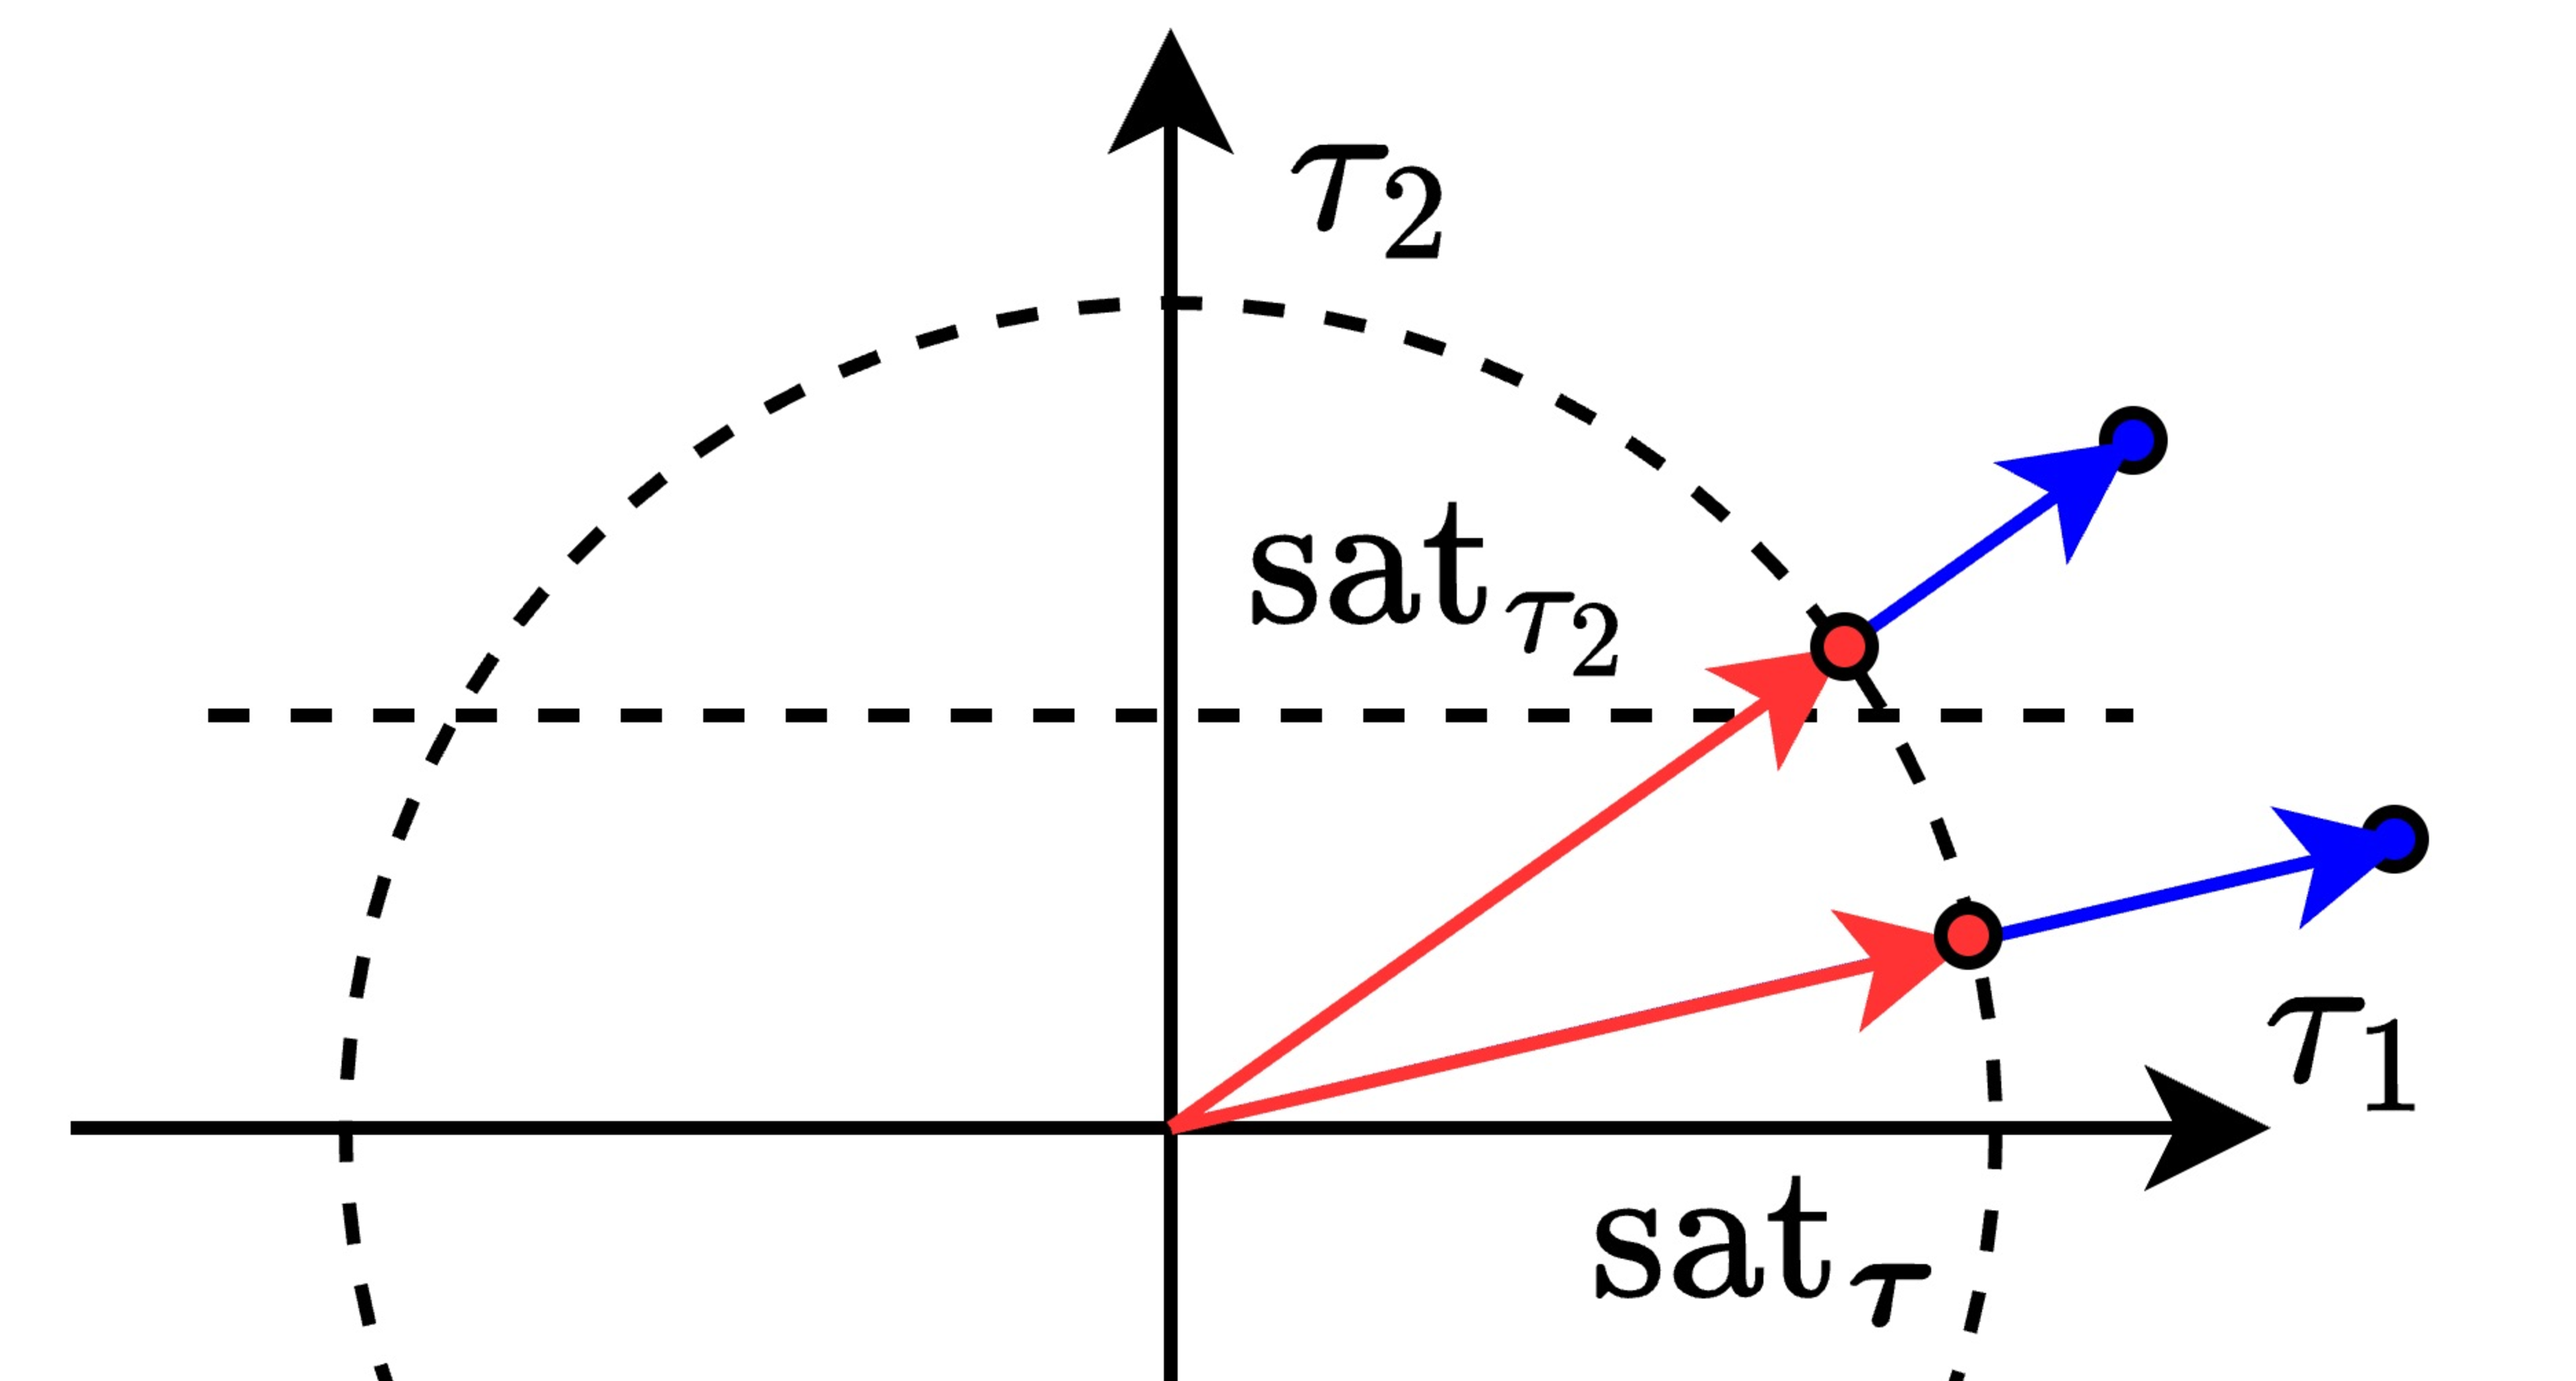
\includegraphics[width=0.45\linewidth]{src/figures/saturation.drawio.pdf}
        \label{fig:robot:sat}
    }
    \caption{Two-link manipulator model and control saturation function.}
    \label{fig:robot}
\end{figure}

% ------------------------------------
% Robot Model Parameters
% -----------------------------------
\begin{table}[t]
    \renewcommand{\arraystretch}{1.3}
    \caption{Two-link manipulator parameters of $p\textsuperscript{th}$ link.}
    \centering
    \begin{tabular}{c m{6.5em} c c c }
    % \begin{tabular}{c c c c c}
    \hline
    \textbf{Symbol} & \textbf{Description} & \textbf{Link 1} & \textbf{Link 2} \\
    \hline
    \hline 
    $m_p$ & Mass & 2.465 (kg) & 2.465 (kg) \\
    \hline
    $l_p$  & Length & 0.2 (m) & 0.18 (m) \\
    \hline
    ${l_c}_p$ & Center of mass & 0.139 (m) & 0.087 (m) \\
    \hline
    $b_p$   & Viscous friction coef. &  0.1 (Nms) & 0.1 (Nms) \\
    \hline
    ${f_c}_p$  & Coulomb friction coef. &  0.24 (Nm) & 0.24 (Nm) \\
    \hline
    ${f_s}_p$  & Static friction coef. &  0.3 (Nm) & 0.2 (Nm) \\
    \hline
    $I_p$  & Inertia & 0.069 (kgm\textsuperscript{2}) & 0.015 (kgm\textsuperscript{2}) \\
    \hline
    \end{tabular}
    \label{table:system:params}
\end{table}

% ------------------------------------
% Reference Trajectory
% ------------------------------------
The desired trajectory for $\q=[q_1,q_2]^\top $ was generated using fifth-order polynomial functions $\mypoly^5(\mv{x}_1,\mv{x}_2,t_f,t)$, to satisfy the initial $\mv{x}_1$ and final $\mv{x}_2$ angle conditions and zero velocities of the joints, where $t_f$ is the time duration.
The desired trajectory is defined as follows:
\begin{equation}
    \qd(t) 
    \!=\! 
    \begin{bmatrix}
        {q_d}_1\\{q_d}_2
    \end{bmatrix}
    \!=\!
    \begin{cases}
    \mypoly^5({\qd}_0,{\qd}_1,t_f,t),
        \!&\!
        \text{if } 0\le t < t_f 
        ,
        \\
    \mypoly^5({\qd}_1,{\qd}_2,t_f,t-t_f),
        \!&\!
        \text{if } t_f\le t < 2t_f 
        ,
        \\
    \mypoly^5({\qd}_2,{\qd}_1,t_f,t-2t_f),
        \!&\! 
        \text{if } 2t_f\le t < 3t_f 
        .
        \\
    \mypoly^5({\qd}_1,{\qd}_0,t_f,t-3t_f),
        \!&\!    
        \text{if } 3t_f\le t < 4t_f 
        ,
        \\
    \end{cases}
    \label{eq:desired trajectory}
\end{equation}
where ${\qd}_0:=\left(-\tfrac{1}{2}\pi,0\right)^\top$, ${\qd}_1:=\left(\tfrac{1}{4}\pi,-\tfrac{1}{2}\pi\right)^\top$, ${\qd}_2:=\left(-\tfrac{1}{4}\pi,\tfrac{1}{4}\pi\right)^\top$, and $t_f=3$ s.
To demonstrate the learning capability of NN, the desired trajectory was applied twice; let us call the first and second iterations of the reference trajectory as Episode $1$ and Episode $2$, respectively.

% However, since the NN's weights are initialized randomly, large reference trajectories should be avoided to mitigate the effect of initial poor performance of the controller.
% Hence, the reference trajectory was applied $2$ times by proportionally increasing the amplitude of the desired trajectory to the original ${\qd}_i,\ \forall i\in\{1,2\}$.
% Let us call the $i\textsuperscript{th}$ iteration of the reference trajectory as Episode $i,\ \forall i\in\{1,2\}$.

% ------------------------------------
% Control Input Saturation
% ------------------------------------
To demonstrate the effectiveness of the proposed CoNAC to handle the combination of the convex input constraints, the saturation function is defined to project the control input onto following convex domain $\Theta_{\mysat}:=\left\{\Theta_{\mysat, {\rbu}}\cap\Theta_{\mysat, {\tau_2}}\right\}$ as depicted in Fig.~\ref{fig:robot:sat}, where
%
\begin{subequations}
    \begin{align}
        \Theta_{\mysat, {\rbu}}
        :=&
        \left\{
            \rbu
            \mid
            \norm{\rbu} \le 
            10
            % \overline\tau
        \right\}
        \label{eq:sat:norm}
        ,
        \\
        \Theta_{\mysat, {\tau_2}}
        :=&
        \left\{
            \tau_2
            \mid
            \vert{\tau_2}\vert \le 
            2.5
            % \overline\tau_2
        \right\}
        .
        \label{eq:sat:tau2}
    \end{align}
    \label{eq:sat}
\end{subequations}
%
These domains \eqref{eq:sat:norm} and \eqref{eq:sat:tau2} can be physically interpreted as a combination of the voltage source limitation of the actuators and the torque limitation of the second link actuator, respectively.

\hfill

% ------------------------------------
% Comparative Study
% ------------------------------------
For a comparative study, we implemented 3 controllers.
The properties of the controllers are summarized in Table~\ref{table:controllers}.

% ------------------------------------
% Controllers: CoNAC 
% ------------------------------------
\subsubsection*{Controller 1: (C$_1$) CoNAC; proposed}

To handle the input saturation, the proposed CoNAC was implemented with the input bound constraint for second link $c_{\overline\tau_2}$ and $c_{\underline\tau_2}$ \eqref{eq:cstr:input:bound} and the nonlinear input norm constraint $c_{\rbu}$ \eqref{eq:cstr:input:norm}, as follows:
\begin{equation}
    c_{\overline\tau_2}     
    =
    \tau_2-\overline\tau_2
    \le 0
    ,
    \;
    c_{\underline\tau_2} 
    =
    \underline\tau_2-\tau_2
    \le 0
    ,
    \;
    c_{\rbu}
    =
    \tfrac{1}{2}
    (
        \norm{\rbu}-\overline\tau
    )^2 
    <0
    ,
    \label{eq:sim:cstr:CoNAC}
\end{equation}
where $\overline\tau_2=-\underline{\tau}_2=2.5$ are the absolute bound of the second link actuator, and $\overline\tau=10$ is the maximum feasible norm of the control input.
Hence, (C$_1$) is possible to use full capability of the actuator.
The weight constraints $c_{\theta_i},\ \forall i\in[0,\cdots,k]$ were also considered in the CoNAC.
As described in \eqref{eq:control:est}, the control input is equal to the output of the NN, and the adaptation law is defined in \eqref{eq:adaptation law}.

The update rate of the Lagrange multipliers was set to $\beta_{\theta_i}=10^{-3},\ \forall i\in[0,\cdots,k]$, and $\beta_{\rbu}=10$ and $\beta_{\overline{\tau}_2}=\beta_{\underline{\tau}_2}=10^{3}$.

% ------------------------------------
% Controllers: Aux. system in CoNAC-AUX
% ------------------------------------
\subsubsection*{Controller 2: (C$_2$) CoNAC with auxiliary system}

On the other hand, the existing auxiliary system \cite{Esfandiari:2014aa,Karason:1994aa,Esfandiari:2015aa} was used to compare with the proposed (C$_1$).
The auxiliary system is defined as $\ddtt{\mv\zeta} = \mm{A}_\zeta \mv{\zeta} + \mm{B}_\zeta \Delta\rbu,\ \mv{\zeta}\vert_{t=0} = \mv{0}_{2\times1}$, where $\mv{\zeta}\in\R^n$ denotes the auxiliary state, $\mm{A}_\zeta\in\R_{<0}^{n\times n}$, and $\mm{B}_\zeta\in\R^{n\times n}$.
The auxiliary state $\mv{\zeta}$ is affected by the saturated control input $\Delta\rbu$, whose entry is defined as $\Delta\tau_{i} = 
\tau_{i}-\max(\underline\tau_i,\min(\overline\tau_i,\tau_i)),\ \forall i\in\{1,2\}$.
Since, the auxiliary system only considers the input bound constraint, $\overline{\tau}_1$ is set to $9.682$ to approximately match the maximum allowable norm of the control input $\overline\tau$, (\ie $\overline{\tau}_1^2+\overline{\tau}_2^2=\overline{\tau}^2$, and $\overline{\tau}_2=2.5$ and $\overline{\tau}=10$).

The auxiliary state are used in the adaptation law \eqref{eq:adap:th:approx} by substituting $\fe$ with $\fe+\mv{\zeta}$.
Hence, the weights are adapted to reduce not only the tracking error $\fe$ but also the auxiliary state $\mv{\zeta}$.

The matrices of the auxiliary system are set to $\mm{A}_\zeta=\mydiag([-10,-10])$ and $\mm{B}_\zeta=\mydiag([10^3,10^3])$, considering the tradeoff between the sensitivity of the control saturation, and the convergence speed.
\MSRY{sensitivity와 convergence에 대해서 더 설명이 필요한가?}

% ------------------------------------
% Controllers: CoNAC with small beta
% ------------------------------------
\subsubsection*{Controller 3: (C$_3$) CoNAC with small $\beta_i$}

To investigate the effect of the update rate of Lagrange multipliers, (C$_3$) was implemented with small $\beta_i$ values, which are set to $\beta_{\rbu}=1$, and $\beta_{\overline{\tau}_2}=\beta_{\underline{\tau}_2}=10^{2}$.
The remaining parameters are the same as (C$_1$).

\hfill

% ------------------------------------
% Controller Parameters
% ------------------------------------
For all controllers ((C$_1$), (C$_2$), and (C$_3$)), the NN input vector ${\q}_n$ was set as ${\q}_n=\left(\q^\top,\dq^\top,\fe^\top,1\right)^\top\in\R^{3n+1}$ with the augmented scalar $1$ included to account for the bias term in the weight matrix. 
The NNs' weights were initialized randomly with uniform distribution in the range of $[-0.1,0.1]$, and the same random seed.
Each NN architecture had two hidden layers with four nodes (\ie $k=2, l_0=6, l_1=4, l_2=4, l_3=2$), and the adaptation gain was set to $\alpha=0.5$.
The filtering matrix $\mm{\Lambda}$ was set to $\mm{\Lambda}=\mydiag([5,15])$.
The sampling rate of the controller was $250$ Hz considering the further real-time implementation, and $1000$ Hz for the simulation.
To emphasize the control input constraint handling capability, the weight constraint parameters were selected sufficiently large (\ie $\overline\wth_0=11, \overline\wth_1=12$, and $\overline\wth_2=13$), avoiding the violation of the weight constraints. 
The readers are referred to the previous papers of the author's \MSRY{ECC, IECON paper} for the demonstration of the capabilities of the proposed CoNAC to address the weight constraints.

The quantitative comparison of the tracking performance was evaluated using the $L_2$-norm of them, (\ie $\sqrt{\int_0^T\norm{h}\,\der t}$, where $h\in\{r_1,r_2\}$ and $T\in\R_{>0}$ denotes the each episode duration time.

% ------------------------------------
% Controller Table
% ------------------------------------
\begin{table}[t]
    \renewcommand{\arraystretch}{1.3}
    \caption{Properties of the controllers used in simulation}
    \label{table:controller}
    \centering
    \begin{tabular}{c l l}
    \hline
        \!&\!\bf{Description}\!&\!\bf{Input Constraint}\!\\
    \hline
    \hline
        (C$_1$) & proposed & $\overline{\tau}=10$ and $\overline{\tau}_2=-\underline{\tau}_2=2.5$ \\
    \hline
        (C$_2$) & aux. sys. & $\overline{\tau}_1=-\underline{\tau}_1=9.682$ and $\overline{\tau_2}=-\underline{\tau_2}=2.5$ \\
    \hline
        (C$_3$) & small $\beta_i$ & $\overline{\tau}=10$ and $\overline{\tau}_2=-\underline{\tau_2}=2.5$ \\
    \hline
    \end{tabular}
    \label{table:controllers}
\end{table}

% ------------------------------------
% Parameter Variation 
% ------------------------------------
% \begin{figure}[!t]      
%     \centering
%     {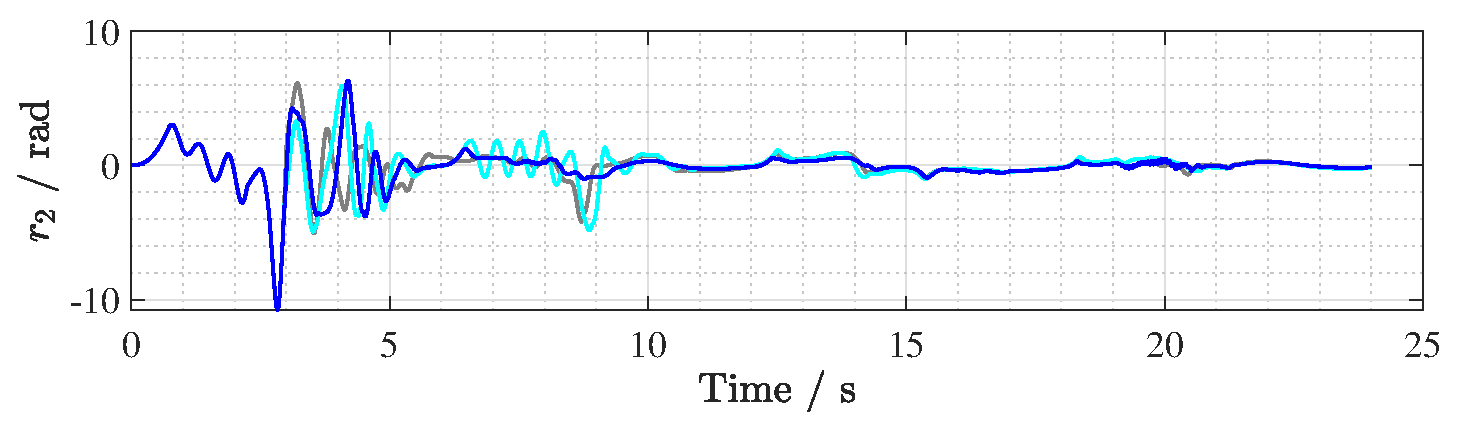
\includegraphics[width=\figSizeOneCol\linewidth]{
%         src/measurement/figures/Fig11.eps
%     }}
% \caption{Box-and-Whisker plot of $L_2$-norms of the tracking performances and control input constraint violations of CoNAC and CoNAC-AUX across various parameter values.}
%     \label{fig:ctrl:result:var}
% \end{figure}


% \begin{table}[!t]
%     \renewcommand{\arraystretch}{1.3}
%     \caption{Quantitative comparison of $L_2$-norms of the tracking performances and control input constraint violations.}
%     \centering
%     \begin{tabular}{c c c c}
%     \hline
%         \!&\!Maximum\!&\!Median\!&\!Minimum\!\\
%     \hline
%     \hline
%     \textbf{CoNAC}\!&\!$11.176\!\times\!10^{-3}$\!&\!$0.590\!\times\!10^{-3}$\!&\!$0.543\!\times\!10^{-3}$ \\
%     \hline
%     \textbf{CoNAC-AUX}\!&\!$0.560\!\times\!10^{-3}$\!&\!$0.552\!\times\!10^{-3}$\!&\!$0.543\!\times\!10^{-3}$ \\
%     \hline
%     \end{tabular}
%     \label{table:ctrl:result:var}
% \end{table}

% ------------------------------------
% Controller Parameters
% ------------------------------------
% \begin{table}[t]
%     \renewcommand{\arraystretch}{1.3}
%     \caption{Parameters of the controllers used in simulation}
%     \label{table:controller:params}
%     \centering
%     \begin{tabular}{c | c c c c c c c c c c c c c c}
%     \hline
%         & $l_0$ & $l_1$ & $l_2$ & $l_3$ & $\alpha$ & $\beta$ & $\overline\theta_0$ & $\overline\theta_1$ & $\overline\theta_2$ & $\overline\tau$ & $\tau_1$ & $\tau_2$ & $\mm{A}_\zeta$ & $\mm{B}_\zeta$ \\
%     \hline
%     \hline
%         \bf{BSC} & \multirow{2}{*}{6} & \multirow{2}{*}{4} & \multirow{2}{*}{4} & \multirow{2}{*}{2} & \multirow{2}{*}{$10^3$} & \multirow{2}{*}{$10^{-4}$} & \multirow{2}{*}{11} & \multirow{2}{*}{12} & \multirow{2}{*}{13} & \multirow{2}{*}{10} & \multirow{2}{*}{11} & 0.5 & & \\
%     % \hline
%         \bf{CoNAC-AUX} &  & & & & & & & & & & & 0.5 & $[20,0;0,20]$ & $[10,0;0,10]$ \\
%     \hline
%     \end{tabular}
% \end{table}

\begin{figure*}[t]
  \centering
    \subfloat[Tracking result of $q_1$.]{
      \includegraphics[width=\figSizeTwoCol\linewidth]
      {
        % src/script_simulation/figures/compare/Fig10.eps
        src/script_simulation/figures/compare/Fig1.eps
      }%
      \label{fig:ctrl:result:q1}}
    \hfill
    \subfloat[Tracking result of $q_2$.]{
      \includegraphics[width=\figSizeTwoCol\linewidth]
      {
        % src/script_simulation/figures/compare/Fig11.eps
        src/script_simulation/figures/compare/Fig2.eps
      }%
      \label{fig:ctrl:result:q2}}
    \vfill
      \subfloat[Control input $\tau_1$.]{
        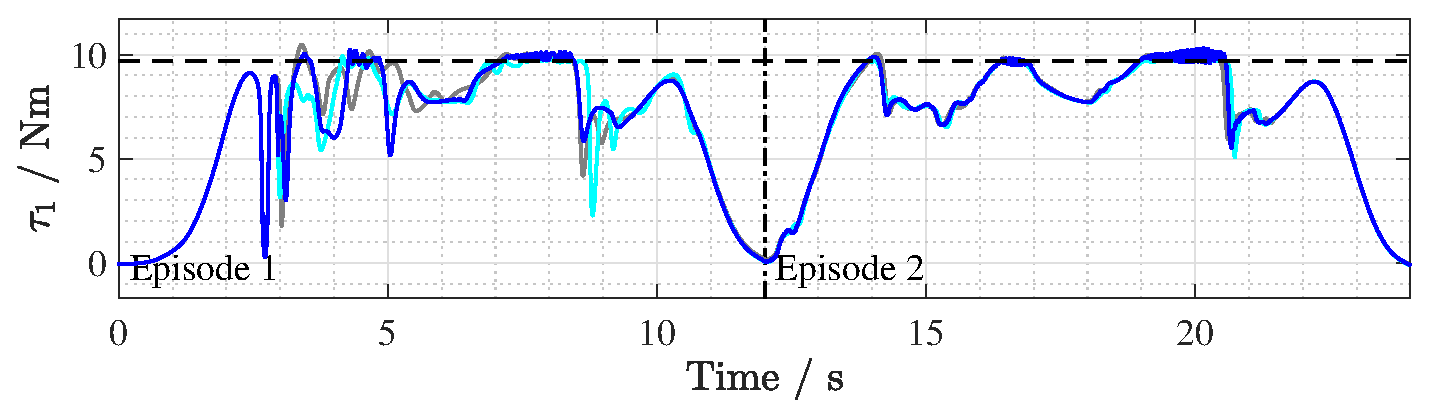
\includegraphics[width=\figSizeTwoCol\linewidth]
        {
            src/script_simulation/figures/compare/Fig3.eps
        }%
        \label{fig:ctrl:result:tau:1}}
    \hfill
      \subfloat[Control input $\tau_2$.]{
        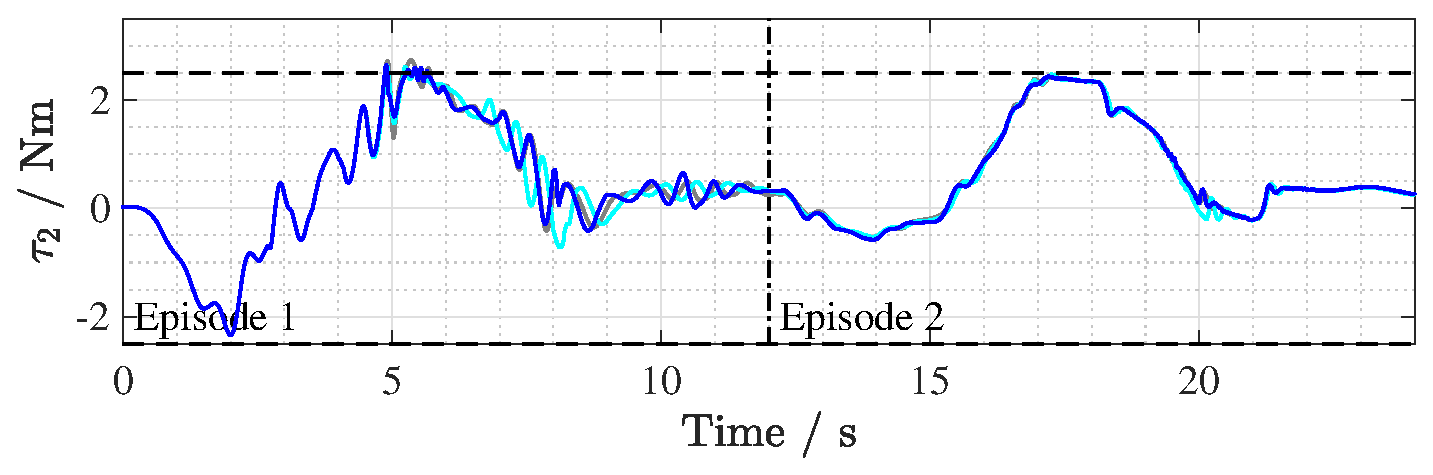
\includegraphics[width=\figSizeTwoCol\linewidth]
        {
            src/script_simulation/figures/compare/Fig4.eps
        }%
        \label{fig:ctrl:result:tau:2}}
        \vfill
    \subfloat[Norm of control input $\tau$.]{
        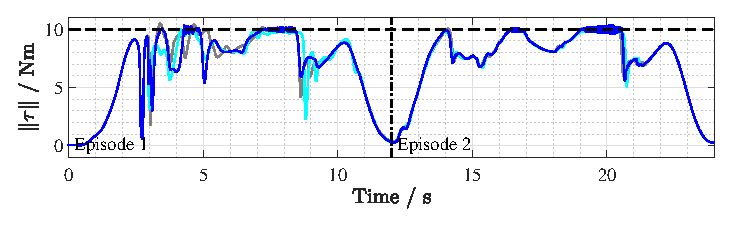
\includegraphics[width=\figSizeTwoCol\linewidth]
        {
            src/script_simulation/figures/compare/Fig5.eps
        }%
        \label{fig:ctrl:result:tau:norm}}
    \hfill
    \subfloat[Norm of weights $\hat\theta_i$.]{
        \includegraphics[width=\figSizeTwoCol\linewidth]
        {
            src/script_simulation/figures/compare/Fig7.eps
        }%
        \label{fig:ctrl:result:weight}}        
    \caption{
  Simulation results of (C$_1$) (blue), (C$_2$) (cyan), (C$_3$) (gray), and reference signal of $\qd$ (red dashed line).
  }
\label{fig:ctrl:result}
\end{figure*}

\begin{figure}[t]
    \centering
    \subfloat[Control input $\tau$ in time interval from $19$ s to $21$ s (bird's eye view).]{
    % \subfloat[Auxiliary states $\mv{\zeta}$ of CoNAC-AUX.]{
        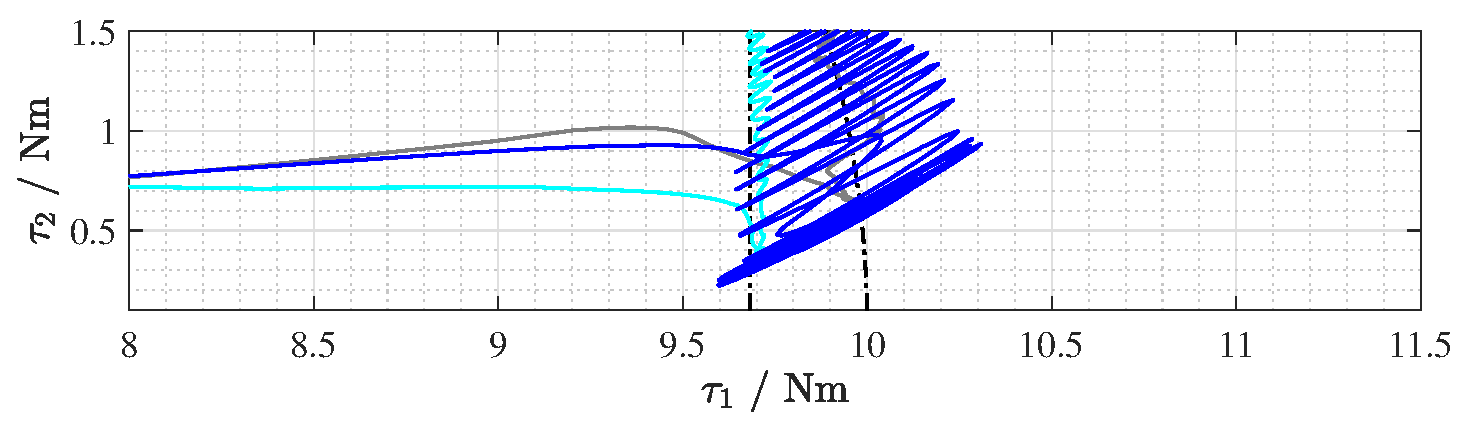
\includegraphics[width=\figSizeOneCol\linewidth]
        {
            src/script_simulation/figures/compare/Fig6.eps
        }%
        \label{fig:ctrl:result:scope:control}}
        \vfill
    \subfloat[Lagrange multipliers $\lambda_j$  in time interval from $19$ s to $21$ s.]{
        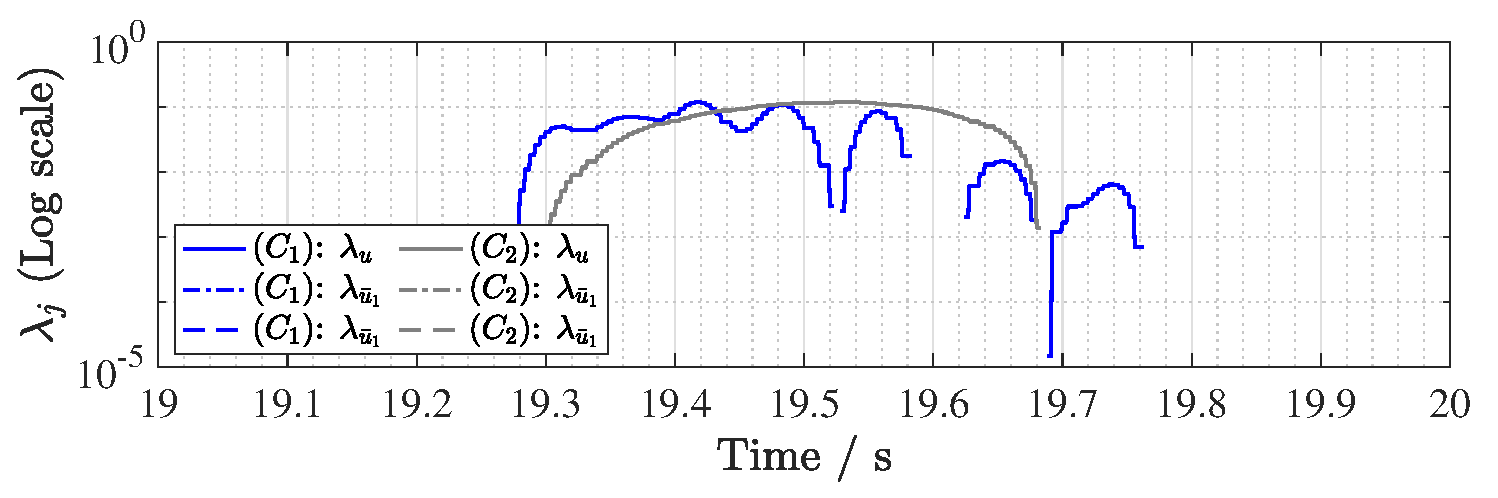
\includegraphics[width=\figSizeOneCol\linewidth]
        {
            src/script_simulation/figures/compare/Fig8.eps
        }%
        \label{fig:ctrl:result:scope:beta}}
        \vfill
    \subfloat[Auxiliary states in time interval from $19$ s to $21$ s.]{
        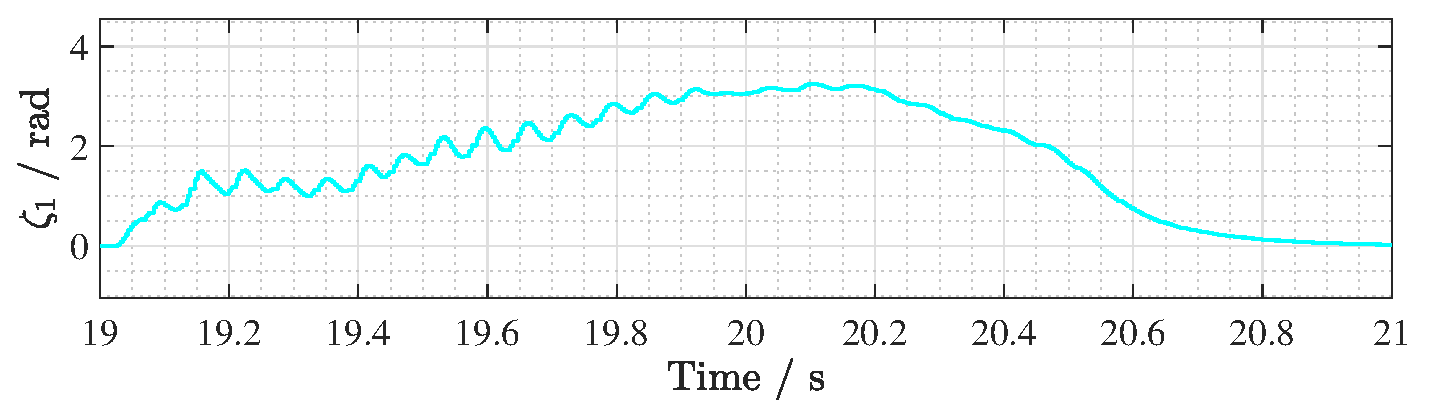
\includegraphics[width=\figSizeOneCol\linewidth]
        {
            src/script_simulation/figures/compare/Fig9.eps
        }%
        \label{fig:ctrl:result:scope:aux}}
  \caption{
    Constraint handling process of (C$_1$) (blue), (C$_2$) (cyan), and (C$_3$) (gray) in time interval from $19$ s to $21$ s.
  }
\label{fig:ctrl:result:scope}
\end{figure}

\begin{figure}[!t]
	\centering
	\includegraphics[width=0.6\linewidth]{
		src/figures/lambda_effect.drawio.pdf
		}
	\caption{
		The effect of Lagrange multiplier $\lambda_{j}$ on the adaptation direction of $\widehat{ \mv{\theta}}_1$.
		The notation ($\cdot'$) and ($\cdot''$) represent two different cases of bigger and smaller Lagrange multiplier, respectively (i.e., $\lambda_{j}' > \lambda_{j}''$).
	}
	% \vspace{1mm}
	\label{fig:lambda_effect}
\end{figure}

% ------------------------------------
% Norm of error in Episode 1: 
% C1 r1 ep1: 0.389
% C1 r2 ep1: 0.426
% C2 r1 ep1: 0.403
% C2 r2 ep1: 0.456
% C3 r1 ep1: 0.370
% C3 r2 ep1: 0.427
% Norm of error in Episode 2: 
% C1 r1 ep2: 0.155
% C1 r2 ep2: 0.066
% C2 r1 ep2: 0.191
% C2 r2 ep2: 0.094
% C3 r1 ep2: 0.141
% C3 r2 ep2: 0.083
% Improvement in Episode 2: 
% C1 r1: 0.602
% C1 r2: 0.845
% C2 r1: 0.527
% C2 r2: 0.793
% C3 r1: 0.619
% C3 r2: 0.805
% ------------------------------------
\begin{table}[!t]
    \renewcommand{\arraystretch}{1.3}
    \caption{Quantitative comparison of performances' $L_2$ norm.}
    \centering
    \begin{tabular}{c c c c c c c}
    \hline
		& \multicolumn{3}{c}{\textbf{Episode 1}}  & \multicolumn{3}{c}{\textbf{Episode 2}} \\
    \hline
	\hline 
		& (C$_1$) & (C$_2$) & (C$_3$) & (C$_1$) & (C$_2$) & (C$_3$) \\
	\hline
		$r_1$ & $0.389$ & $0.403$ & $0.370$ & $0.155$ & $0.191$ & $0.141$ \\ 
	\hline
        $r_2$ & $0.426$ & $0.456$ & $0.427$ & $0.066$ & $0.094$ & $0.083$ \\
	\hline
    \end{tabular}
    \label{tab:sim:L2}
\end{table}

% ------------------------------------
% Tracking Performance
% ------------------------------------
\subsubsection{Tracking Performance}

The simulation results are shown in Fig.~\ref{fig:ctrl:result} and the quantitative comparison of the tracking performance is given in Table~\ref{tab:sim:L2}.
Across the two episodes, all controllers enhanced their tracking performances about 
$60.2 \%$ for (C$_1$), $52.7 \%$ for (C$_2$), and $61.9 \%$ for (C$_3$) in $L_2$ norm of $r_1$, and $84.5 \%$ for (C$_1$), $79.3 \%$ for (C$_2$), and $80.5 \%$ for (C$_3$) in $L_2$ norm of $r_2$, respectively, as shown in Table~\ref{tab:sim:L2}.
Qualitatively, as described in Fig.~\ref{fig:ctrl:result:q1} and Fig.~\ref{fig:ctrl:result:q2}, the oscillations were suppressed in the second episode, as well.
This results lead to the conclusion that the NNs in all controllers were able to learn the ideal control input $\rbu^*$ properly, by the filtered error $\fe$, despite the fact that $\rbu^*$ was not known in advance.
Moreover, since the learning began from the random initialization of the weights and no prior knowledge of the system, the online learning capability of the proposed CoNAC was demonstrated.

In addition, it is notable that in both episodes, all controllers failed to track the desired trajectory of $q_1$ in time interval from $7.5$ s to $8.5$ for Episode $1$, and from $19.5$ s to $20.5$ s for Episode $2$.
This is because the control inputs were saturated in the time intervals, as shown in Fig.~\ref{fig:ctrl:result:tau:1} and Fig.~\ref{fig:ctrl:result:tau:norm}.
However, 

The tracking performance of CoNAC, (\ie (C$_1$), and (C$_3$)), outperformed (C$_2$) in both episodes, as shown in Table~\ref{tab:sim:L2}.
This is because, (as wil be discussed in Section \ref{sec:sim:constraint}) (C$_1$) was able to use the full capability of the actuator, while (C$_2$) was limited its first link actuator due to the feature of the auxiliary system.

% ------------------------------------
% Control Input Saturation
% ------------------------------------
\subsubsection{Constraint Handling} \label{sec:sim:constraint}

In this section, the constraint handling capability of all controllers are investigated.
First, the weight norm constraints $c_{\theta_i},\ \forall i\in\{0,1,2\}$ were not violated, as shown in Fig.~\ref{fig:ctrl:result:weight}, since the limits $\overline{\theta}_i,\ \forall i\in\{0,1,2\}$ were set sufficiently large.

As shown in Fig.~\ref{fig:ctrl:result:tau:1}, Fig.~\ref{fig:ctrl:result:tau:2}, and Fig.~\ref{fig:ctrl:result:tau:norm}, all controllers satisfied the control input saturation illustrated in Fig.~\ref{fig:robot:sat}, with $c_{\rbu},c_{\overline\tau_2}$ and $c_{\underline\tau_2}$ for (C$_1$) and (C$_3$), and $c_{\overline\tau_1},c_{\underline\tau_1},c_{\overline\tau_2}$, and $c_{\underline\tau_2}$ for (C$_2$), as the weights were adapted to reduce the constraint violations, using Lagrange multipliers $\lambda_j,\ \forall j\in\mathcal{I}$, and auxiliary state $\mv{\zeta}$, respectively.
It is worth to note that the control input constraints were violated repeatedly, since the controllers were implemented in discrete time with a low sampling rate of $250$ Hz.

\hfill

Even though all controllers satisfied the input saturation, (C$_2$) was not able to use the full capability of the actuator, as shown in Fig.~\ref{fig:ctrl:result:scope:control} which shows the bird-eye view of the control input $\rbu$ in time interval from $19$ s to $21$ s.
This is because, as aforementioned, the auxiliary system only considers the input bound constraint, and the control input bound constraint for first link was imposed to approximately match the maximum allowable norm of the control input $\overline\tau$, instead of $c_{\rbu}$.
In contrast, (C$_1$) and (C$_3$) were able to use the full capability of the actuator with the combination of the input bound constraints $c_{\overline\tau_2}$ and $c_{\underline\tau_2}$, and the nonlinear input norm constraint $c_{\rbu}$ which is completely match the feasible domain of the control input $\Theta_{\mysat}$.

\hfill

% zeta
The detail of the constraint handling in the time interval from $19$ s to $21$ s, is now investigated.
First, for (C$_2$), the auxiliary state $\zeta_1$ generated by constraint violation of $c_{\overline\tau_1}$. 
As the weights were adapted to reduce not only $\fe$ but also $\mv{\zeta}$, the constraint violation of $c_{\overline\tau_1}$ was reduced, as shown in Fig.~\ref{fig:ctrl:result:scope:control}.
After the constraint was satisfied, the auxiliary state $\zeta_1$ converged to zero, by the stable state matrix $\mm{A}_\zeta$ in the auxiliary system, \ie $\ddtt\mv{\zeta} = \mm{A}_\zeta \mv{\zeta} + \mm{B}_\zeta \Delta\rbu$ with $\Delta\rbu=\mv{0}_{2\times1}$.


% beta + zeta
For the cases of (C$_1$) and (C$_3$), the Lagrange multipliers $\lambda_{\rbu}$ adjusted the adaptation direction of the weights $\widehat{ \mv{\theta}}_1$ to reduce the constraint violation $c_{\rbu}$, as $\lambda_{\rbu}$ increased by the constraint violations.
% comparison; big, small beta
For more details, the effect of the update rate $\beta_j,\ \forall j\in\mathcal I$ of Lagrange multipliers is shown in Fig.~\ref{fig:lambda_effect} for convex constraint $c_j,\ \forall j\in\mathcal I$ and two different cases of $\lambda_j$.
With the bigger $\lambda_j$, the adaptation of $\widehat{ \mv{\theta}}_1$ is more assertive than that with smaller $\lambda_j$.
This leads to a faster satisfaction of the constraint $c_j,\ \forall j\in\mathcal I$, but this also causes oscillation in the adaptation process.
In Fig.~\ref{fig:ctrl:result:scope:control} and Fig.~\ref{fig:ctrl:result:scope:beta}, $\lambda_j$ of (C$_1$) repeatedly increased and decreased, which indicates that the constraint $c_j,\ \forall j\in\mathcal I$ was satisfied and violated, respectively, in the discrete time implementation.
Besides, with small $\lambda_j$, the adaptation direction of $\widehat{ \mv{\theta}}_1$ is adjusted more conservatively, which leads to a slower satisfaction of the constraint $c_j,\ \forall j\in\mathcal I$, as shown in Fig.~\ref{fig:ctrl:result:scope:control} and the positively existence of $\lambda_j$ in Fig.~\ref{fig:ctrl:result:scope:beta}.
This allows the controller to show a smoother control input.
However, since the weights were adapted to reduce the filtered error $\fe$ while the control input was saturated, the weights were not able to effectively adapt the weights with respect to the filtered error $\fe$.

% ------------------------------------
% Real-time Implementation Set-up
% ------------------------------------
\begin{figure}[t]
    \centering
        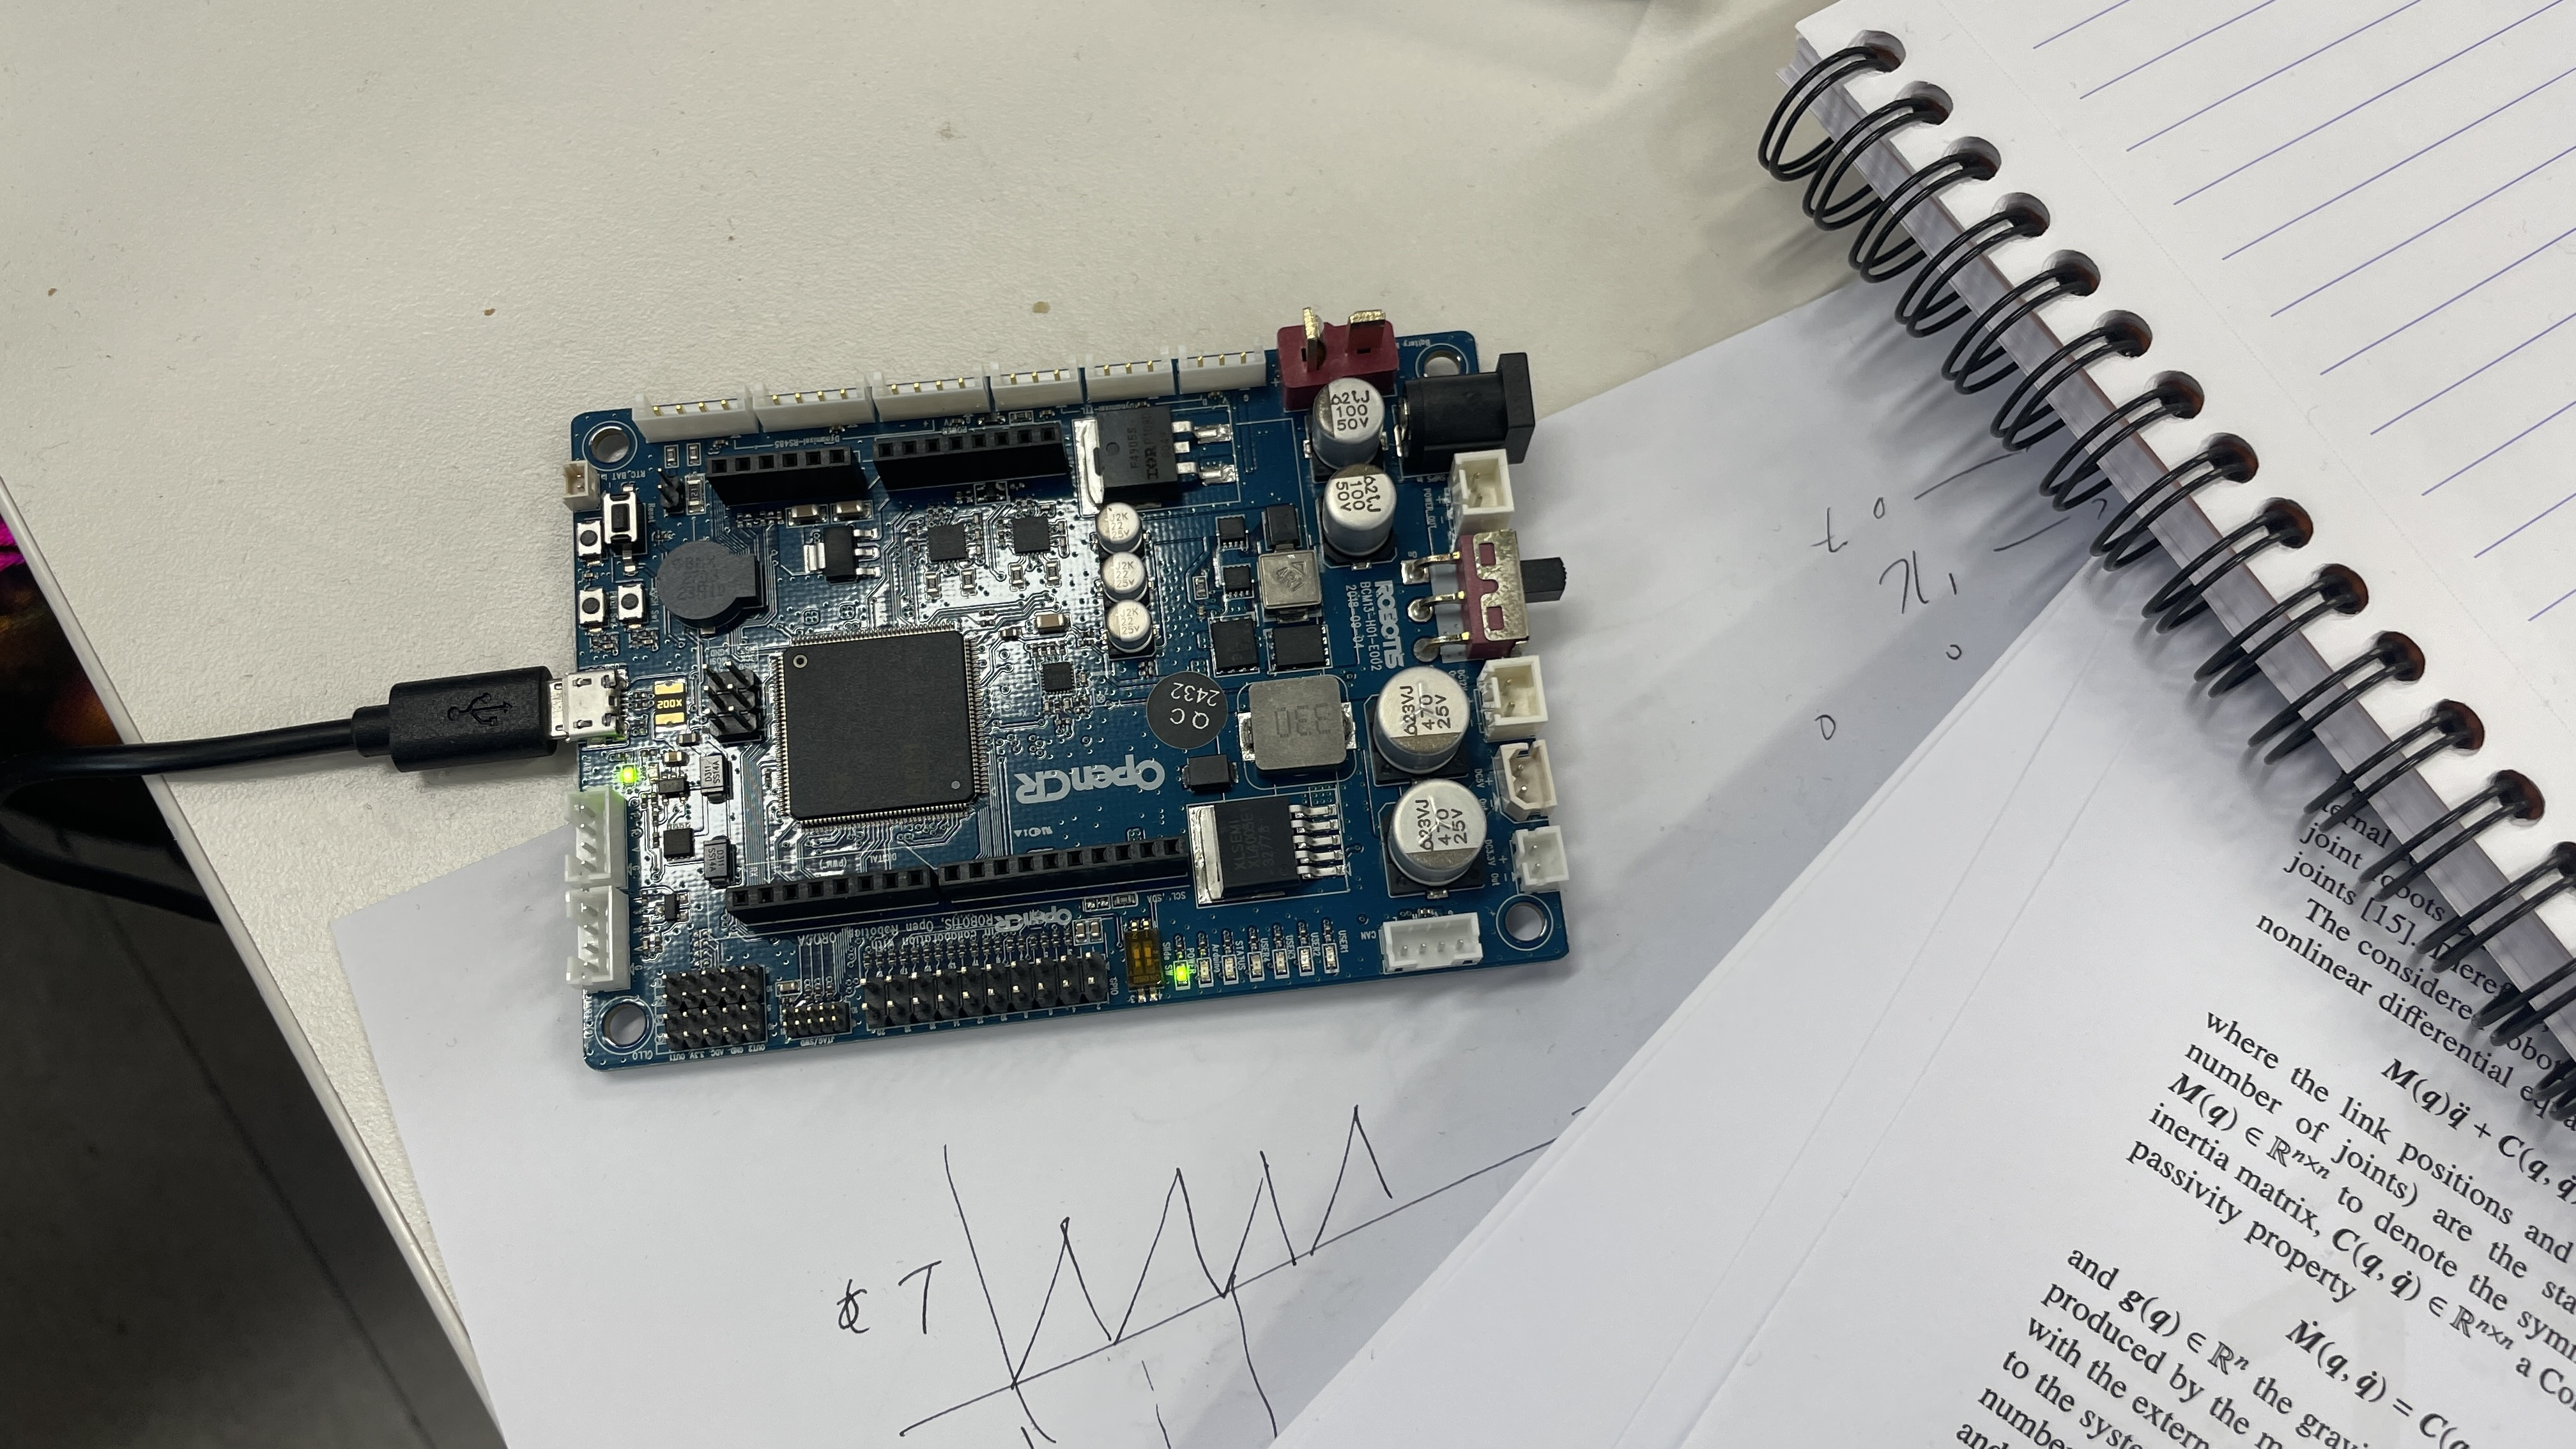
\includegraphics[width=\figSizeOneCol\linewidth]
        {
            fig/exp_set.jpg
        }%
    \caption{
        Robot setup for the real-time experiment.
    }
    \label{fig:ctrl:exp:set}
  \end{figure}

\subsection{Real-time Experiment Validation}

To validate the effectiveness of the proposed CoNAC, a real-time experiment was conducted on a two-link manipulator, as shown in Fig.~\ref{fig:ctrl:exp:set}. 
The OpenCR1.0 \cite{opencr} with a 32-bit ARM Cortex and a 216 MHz clock frequency was used for the real-time implementation.
\color{red}
The experimental setup consisted of a two-link manipulator with a 2-DOF arm, equipped with two @@@@@ servos. 
The servos were controlled using the OpenCR1.0 board, which was connected to a computer via USB. 
The reference trajectory was generated using the same method as in the numerical simulation.
\color{black}
The equal reference trajectory was applied and the parameters of the CoNAC were set to those whose best performance was achieved in the simulation (\ie $\beta=...$).
Additionally, the computational time was measured to validate the effectiveness of the proposed CoNAC in real-time applications.

\begin{figure*}[t]
    \centering
      \subfloat[Tracking result of $q_1$.]{
        \includegraphics[width=\figSizeTwoCol\linewidth]
        {
            src/script_simulation/figures/compare/Fig1.eps
        }%
        \label{fig:ctrl:real:result:q1}}
      % \vfill
      \subfloat[Tracking result of $q_2$.]{
        \includegraphics[width=\figSizeTwoCol\linewidth]
        {
            src/script_simulation/figures/compare/Fig2.eps
        }%
        \label{fig:ctrl:real:result:q2}}
      \vfill
        \subfloat[Control input $\tau_1$.]{
          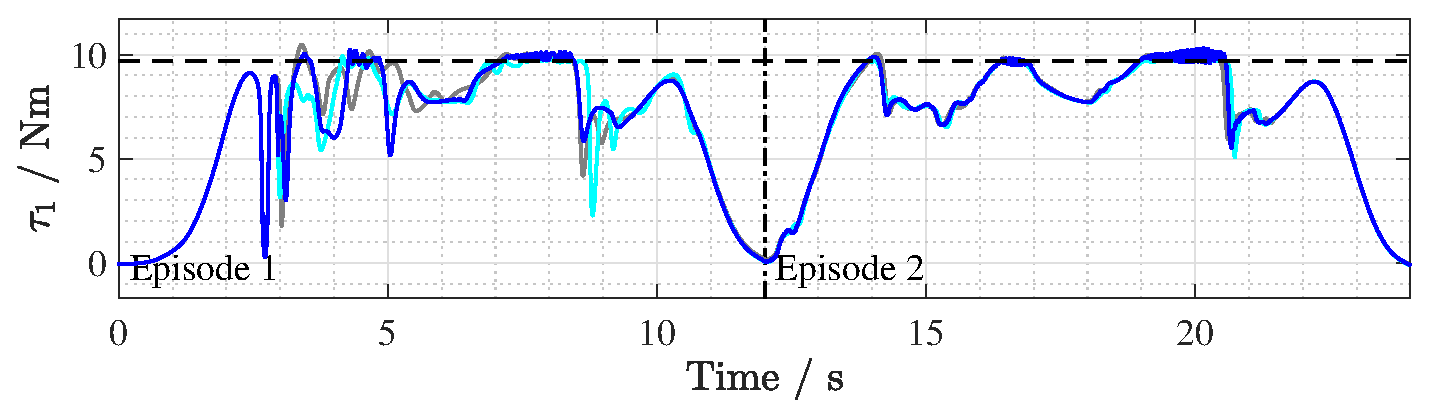
\includegraphics[width=\figSizeTwoCol\linewidth]
          {
            src/script_simulation/figures/compare/Fig3.eps
          }%
          \label{fig:ctrl:real:result:tau:1}}
      % \vfill
        \subfloat[Control input $\tau_2$.]{
          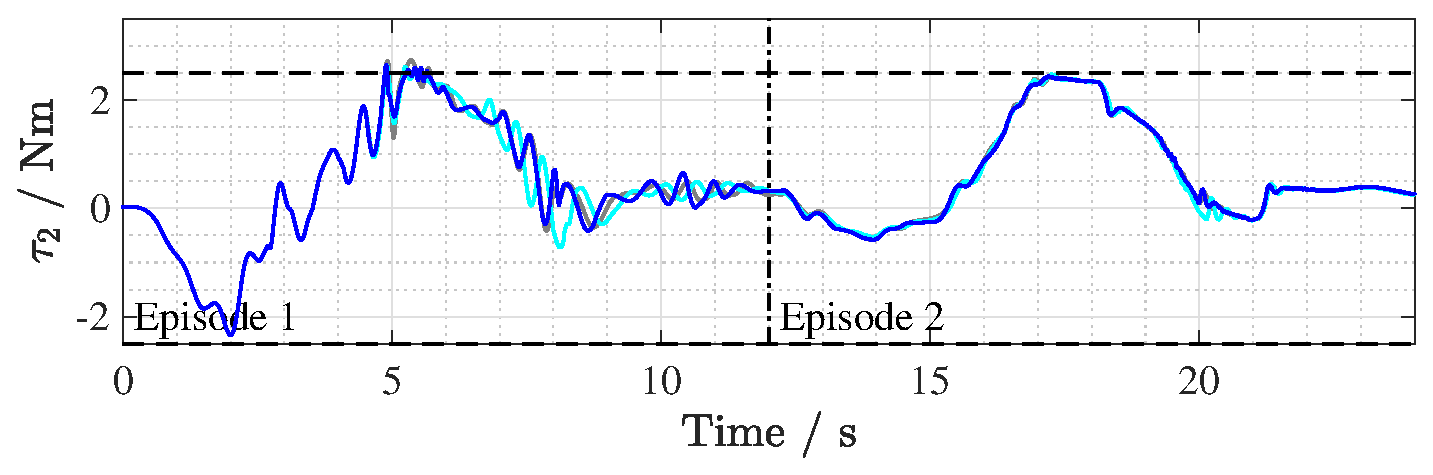
\includegraphics[width=\figSizeTwoCol\linewidth]
          {
            src/script_simulation/figures/compare/Fig4.eps
          }%
          \label{fig:ctrl:real:result:tau:2}}
          \vfill
      \subfloat[Norm of weights $\hat\theta_i$.]{
          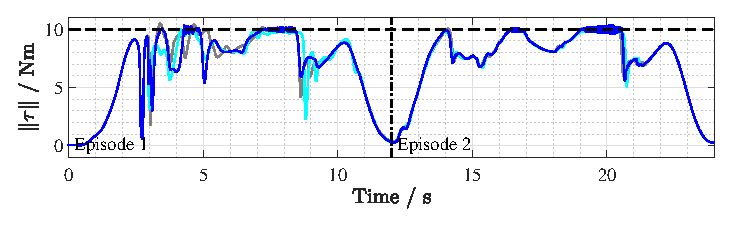
\includegraphics[width=\figSizeTwoCol\linewidth]
          {
            src/script_simulation/figures/compare/Fig5.eps
          }%
          \label{fig:ctrl:real:result:opt:norm}}
          % \vfill
      \subfloat[Lagrange multipliers $\lambda_j$ in logarithmic scale.]{
          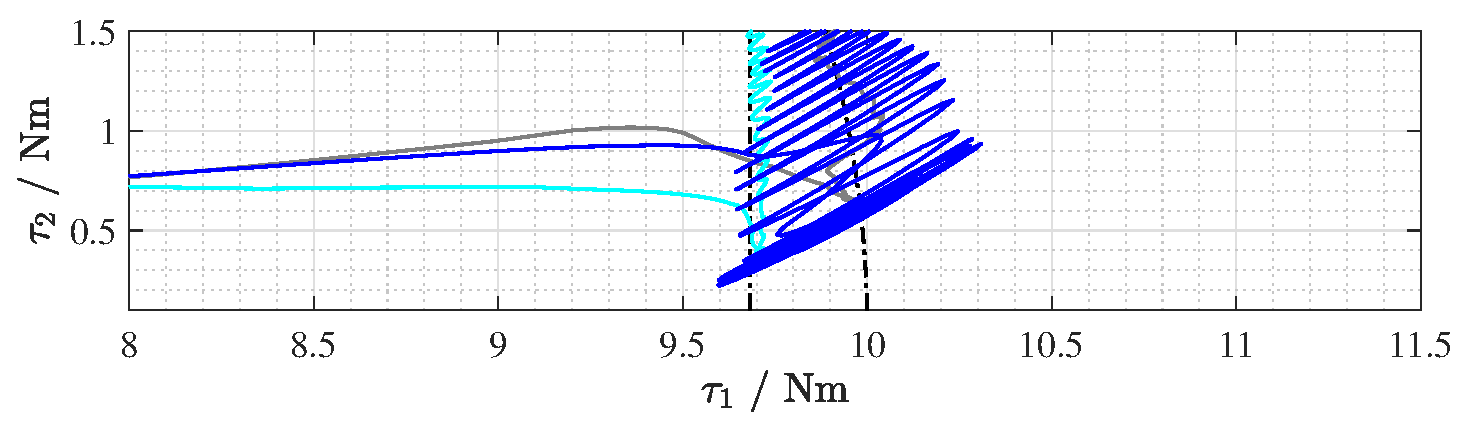
\includegraphics[width=\figSizeTwoCol\linewidth]
          {
            src/script_simulation/figures/compare/Fig6.eps
          }%
          \label{fig:ctrl:real:result:opt:multiplier}}
          \vfill
      \subfloat[Auxiliary states $\mv{\zeta}$ of CoNAC-AUX.]{
          \includegraphics[width=\figSizeTwoCol\linewidth]
          {
            src/script_simulation/figures/compare/Fig7.eps
          }%
          \label{fig:ctrl:real:result:opt:zeta}}
          % \vfill
      \subfloat[Control input $\tau$ in time interval from $1$ s to $3$ s (bird's eye view).]{
          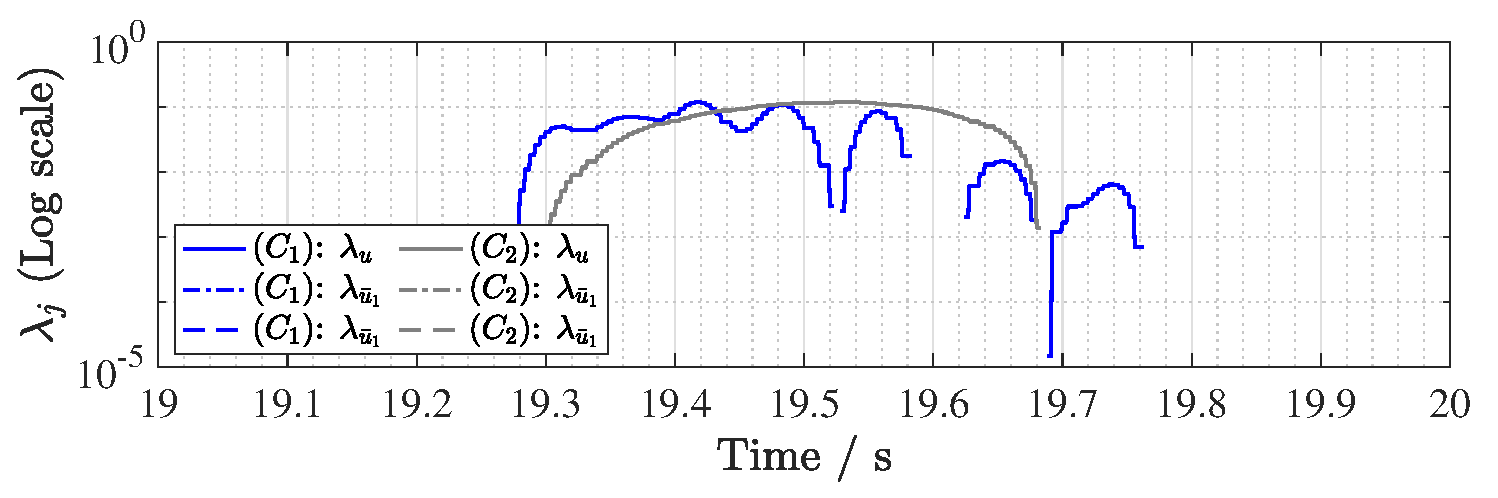
\includegraphics[width=\figSizeTwoCol\linewidth]
          {
            src/script_simulation/figures/compare/Fig8.eps
          }%
          \label{fig:ctrl:real:result:control}}
    \caption{
    Simulation results of the CoNAC (blue) and CoNAC-AUX (cyan), and reference signal of $\qd$ (red dashed line).
    }
  \label{fig:ctrl:real:result}
  \end{figure*}

\begin{figure}[t]
    \centering
        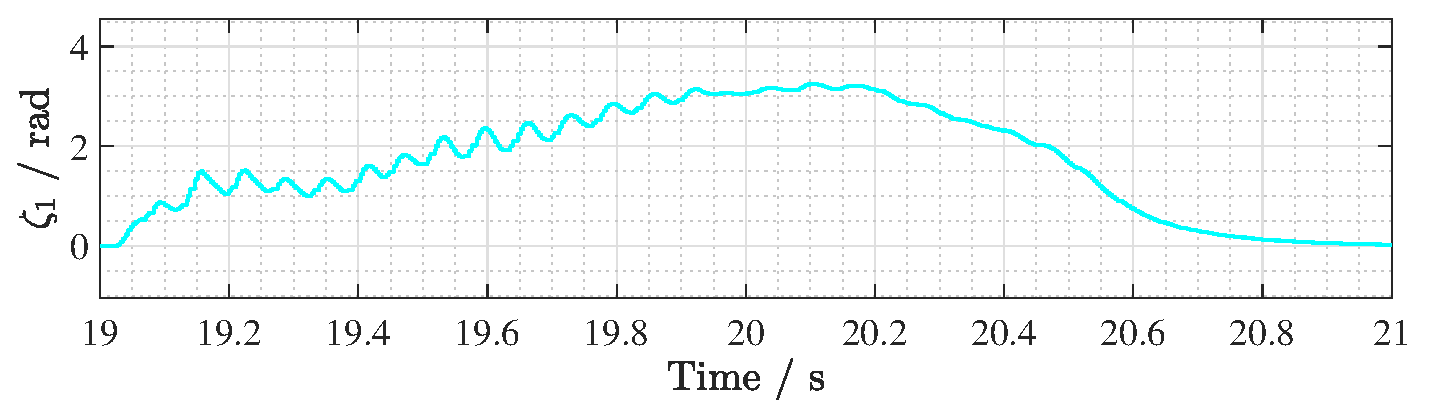
\includegraphics[width=\figSizeOneCol\linewidth]
        {
            src/script_simulation/figures/compare/Fig9.eps
        }%
    \caption{
        Computational time of CoNAC and CoNAC-AUX. 
    }
    \label{fig:ctrl:real:result:cmp:time}
  \end{figure}

\subsubsection{Tracking Performance and Constraint Handling}

% ----------------------------
% tracking performance + learning
% ----------------------------
The tracking result of the real-time experiment is shown in Fig.~\ref{fig:ctrl:real:result}.

% ----------------------------
% cosntraint handling
% ----------------------------

% ----------------------------
% computational time
% ----------------------------
\subsubsection{Computational Time}
is shown in Fig.~\ref{fig:ctrl:real:result:cmp:time}. The computational time of CoNAC was 0.5 ms, which is less than the sampling time of 4 ms. 
This indicates that the proposed CoNAC can be implemented in real-time applications. 

%  SECTION CONCLUSION ======================================
\section{Conclusion}\label{sec:conclusion}

This paper presented a constrained optimization-based neuro-adaptive controller (CoNAC) for the uncertain Euler-Lagrange system, addressing both weight norm and input constraints through a rigorous optimization framework. The stability of the proposed controller was analyzed using Lyapunov theory, ensuring that the system maintained bounded tracking and estimation errors under real-time adaptation.

The controller effectively incorporated both the input (bound or norm) constraint and the weight norm constraint, ensuring that both actuator limitations and neural network weights were kept within predefined bounds. By formulating these constraints as part of the optimization process, CoNAC ensured that the weights converged in a way that satisfied the Karush-Kuhn-Tucker (KKT) conditions, guaranteeing optimality and stability.

Simulation results validated the superior performance of CoNAC compared to conventional methods, such as DNN-BSC and DNN-BSC-A. CoNAC not only handled complex input constraints but also managed the weight norm constraints rigorously, leading to improved tracking accuracy and stability without notable oscillations.

Future work may extend this approach to address constraints on both the system inputs and states, further enhancing the flexibility and robustness of neuro-adaptive control systems using constrained optimization.

%% The Appendices part is started with the command \appendix;
%% appendix sections are then done as normal sections
\appendix

\section{Input Constraint Candidates}\label{sec:appen:cstr} 

This section introduces potential weight and input constraints that can be used in the proposed neuro-adaptive controller. 

\subsection{Input Bound Constraint}\label{sec:appen:cstr:input:bound}

Most physical systems have control input limits due to electrical and mechanical limitations. These are expressed as $\boldsymbol{c}_{\overline \tau}:= [c_{\overline \tau_i}]_{i\in[1,\cdots,n]}$ and $\boldsymbol{c}_{\underline\tau}:= [c_{\underline\tau_i}]_{i\in[1,\cdots,n]}$, where
\begin{equation}
    \begin{aligned}
        c_{\overline \tau_i}=\tau_{(i)} - {\tau_{\overline \tau_i}} \le 0
        ,
        \quad
        c_{\underline\tau_i}={\tau_{\underline\tau_i}}-\tau_{(i)} \le 0
        ,
    \end{aligned}
    \label{eq:cstr:input:bound}
\end{equation}
with $\tau_{\overline \tau_i}$ and $\tau_{\underline\tau_i}$ representing the maximum and minimum control input bounds, respectively.
% The corresponding Lagrange multipliers are $\lambda_{u_j,i},\ \forall j\in[M,m]$. 
The gradients of $\boldsymbol{c}_{\overline \tau}$ and $\boldsymbol{c}_{\underline\tau}$ with respect to $\estwth$ are given by
\begin{equation}
    \begin{aligned}
        \pptfrac{\boldsymbol c_{\overline \tau}}{\estwth}
        =& 
        \begin{bmatrix}
            \pptfrac{c_{\overline \tau_1}}{\estwth}^\top \\
            \vdots \\
            \pptfrac{c_{\overline \tau_n}}{\estwth}^\top
        \end{bmatrix}
        = 
            +\pptfrac{\estNN}{\estwth}
        %     \\
        % =&
        =
        +
        \begin{bmatrix}
            (I_{l_{k+1}}\otimes \estact_{k}^\top)&
            \!\cdots\! &
            (
                \cdot
            )
        \end{bmatrix} 
        \in
        \mathbb R^{n\times \Xi}
        , 
        \\
        \pptfrac{\boldsymbol c_{\underline\tau}}{\estwth}         
        =
        & 
        \begin{bmatrix}
            \pptfrac{c_{\underline\tau_1}}{\estwth}^\top \\
            \vdots \\
            \pptfrac{c_{\underline\tau_n}}{\estwth}^\top
        \end{bmatrix}
        = 
        -\pptfrac{\estNN}{\estwth}
        % \\
        % =&
        =
        -\begin{bmatrix}
            (I_{l_{k+1}}\otimes \estact_{k}^\top)&
            % V_k^\top \phi_{k}' (I_{l_{k}}\otimes  \phi_{k-1}^\top)&
            \!\cdots\! &
            (
                \cdot
            )
        \end{bmatrix} 
        \in
        \mathbb R^{n\times \Xi}
        .
    \end{aligned}
    \label{eq:cstr:input:bound:grad}
\end{equation}

\subsection{Input Norm Constraint}\label{sec:appen:cstr:input:norm}

Consider the control input $\tau$ as the torque of each actuator corresponding to its generalized coordinate. Since torque is typically linearly proportional to current, actuators that share a common power source are often subject to total current limitations. This can be captured by the following inequality constraint: 
\begin{equation}
    c_{\rbu}=\norm{\mv{\tau}}^2 -\overline\tau^2  \le 0
    ,
    \label{eq:cstr:input:norm}
\end{equation}
with $\overline\tau\in\R_{>0}$ denoting the maximum allowable control input magnitude. This input norm constraint is also commonly applied in current and torque control problems for electric motors \cite{Choi:2024aa}.
% The corresponding Lagrangian multiplier is $\lambda_{u_b}$. 
The gradients of $c_{\rbu}$ with respect to $\estwth$ are given by
\begin{equation}
    \pptfrac{\boldsymbol c_{\rbu}}{\estwth}
    \!=\! 
    \textstyle\sum_{i=1}^n 2\tau_{(i)} 
    \left(
        \myrow_i
        (
            \pptfrac{\estNN}{\estwth}
        )
    \right)^\top  
    \!=\! 
    {\pptfrac{\estNN}{\estwth}}^\top
    \mv{\tau}
    % \tau^\top (I_{l_{k+1}}\otimes \estNN_k^\top)
    \in \mathbb R^{\Xi}.
    \label{eq:cstr:input:norm:grad}
\end{equation}
It should be noted that constraints \eqref{eq:cstr:input:bound} and \eqref{eq:cstr:input:norm} can be imposed simultaneously, as their gradients \eqref{eq:cstr:input:bound:grad} and \eqref{eq:cstr:input:norm:grad} are linearly independent, satisfying the LICQ condition.

%% If you have bib database file and want bibtex to generate the
%% bibitems, please use
%%
\bibliographystyle{elsarticle-harv} 
\bibliography{\template/refs}

%% else use the following coding to input the bibitems directly in the
%% TeX file.

%% Refer following link for more details about bibliography and citations.
%% https://en.wikibooks.org/wiki/LaTeX/Bibliography_Management


% \bibliographystyle{elsarticle-harv}
% % \bibliography{}
% \bibliography{\template/refs}


\end{document}

\endinput
%%
%% End of file `elsarticle-template-harv.tex'.


